\documentclass{beamer}
\usetheme{ut}
\usepackage{pgf}
%\usepackage{slashbox}
\usepackage{calc}
\usepackage{tikz}
\usetikzlibrary{positioning}

\pgfdeclareimage[width=.9\textwidth]{signaling-schematic}{images/signaling_schematic}
\pgfdeclareimage[width=.6\textwidth]{activity00}{images/protein_activity00}
\pgfdeclareimage[width=.6\textwidth]{activity01}{images/protein_activity01}
\pgfdeclareimage[width=.6\textwidth]{activity02}{images/protein_activity02}
\pgfdeclareimage[width=.6\textwidth]{activity03}{images/protein_activity03}
\pgfdeclareimage[width=.6\textwidth]{activity04}{images/protein_activity04}
\pgfdeclareimage[width=.9\textwidth]{ta}{images/ta}
\pgfdeclareimage[width=.8\textwidth]{case-study}{images/mapk_model_egf4}
\pgfdeclareimage[width=.9\textwidth]{grafico-ruvido}{images/10levels}
\pgfdeclareimage[width=.9\textwidth]{grafico-liscio}{images/100levels}
\pgfdeclareimage[width=.9\textwidth]{animo-logo}{images/animo_logo}
\pgfdeclareimage[width=.3\textwidth]{animo-qrcode}{images/animo_site_qrcode}
\pgfdeclareimage[width=.9\textwidth]{animo-user-interface}{images/animo_user_interface}
\pgfdeclareimage[width=.75\textwidth]{animo-workflow}{images/animo_simulation_workflow}
\pgfdeclareimage[width=2cm]{activity-legend}{images/activity_legend}
\pgfdeclareimage[width=.9\textwidth]{ta-reactant-centered}{images/Reactant-centered}

\newenvironment{changemargin}[2]{%
\begin{list}{}{%
\setlength{\topsep}{0pt}%
\setlength{\leftmargin}{#1}%
\setlength{\rightmargin}{#2}%
\setlength{\listparindent}{\parindent}%
\setlength{\itemindent}{\parindent}%
\setlength{\parsep}{\parskip}%
}%
\item[]}{\end{list}}


\newcommand{\titledFrameImage}[2]{
\begin{frame}{#1}
%\begin{changemargin}{-1cm}{-1cm}
\begin{center}
\includegraphics[width=108mm,height=\textheight,keepaspectratio]{#2}
\end{center}
%\end{changemargin}
\end{frame}
}

\newcommand{\plainFrameImage}[1]{
\begin{frame}[plain]
%\begin{changemargin}{-1cm}{-1cm}
\begin{center}
\includegraphics[width=108mm,height=76mm,keepaspectratio]{#1}
\end{center}
%\end{changemargin}
\end{frame}
}

\newcommand{\maxFrameImage}[1]{
    %\setbeamertemplate{background}[ut][]
    \begin{frame}[plain]
        \begin{changemargin}{-2cm}{-2cm}
        \begin{center}
            \includegraphics[width=\paperwidth,height=\paperheight,keepaspectratio]{#1}
        \end{center}
        \end{changemargin}
    \end{frame}
    %\setbeamertemplate{background}[ut][0]
}

\makeatletter
\setbeamertemplate{footline}
{%
 \hspace{\beamer@leftmargin}
\hspace{-4.6ex}

\includegraphics[height=4mm,page=1]{beamerthemeutresources}
\hspace*{2ex}
\hfill
\begin{beamercolorbox}[ht=2cm,wd=9cm,sep=0cm]{fg=black,bg=red}
\hfill
%  [ \insertshortauthor, \insertshortinstitute\ ]
\tiny\insertfootlinetext
\hspace{2ex}
%\tiny\insertframenumber/\inserttotalframenumber
\hspace*{\beamer@rightmargin}
\vspace*{1.5ex}
\end{beamercolorbox}
}
\makeatother

\title{Setting parameters for biological~models with ANIMO}
\author{\small \underline{Stefano~Schivo}, Jetse~Scholma, Marcel~Karperien, Janine~N.~Post, Jaco~van~de~Pol, Rom~Langerak}
\institute{University of Twente,\\ Enschede, The Netherlands}
\footlinetext{ANIMO \--\ Analysis of Networks with Interactive MOdeling}
\date[SynCoP2014]{SynCoP 2014}
%\date{}

% A che domande biologiche rispondiamo con ANIMO
% Approccio: interaction-based, discrete levels, sottolinea la concorrenza
% Magari evitare di mostrare modelli TA
% Come funziona la modellazione in ANIMO: topologia, scenari, parametri (con esempi) (tipo Gene?)
% Come funziona l'esperimento in silico (simulazione, model checking, grafici sim+data, slider)
% Demo breve
% Piani futuri: generazione di ipotesi, model checking (esempi??), high-performance analysis
\listfiles

\begin{document}

\maketitle

  \frame{ \frametitle{Signalling Pathways}
    \begin{center}
      %\pgfuseimage{pathway-semplificato}
      \begin{minipage}[c]{.9\textwidth}%
	\pgfuseimage{signaling-schematic}\\[-1ex]%
	{\tiny Credit: National Science Foundation}%
      \end{minipage}
    \end{center}
% Cells receive external signals (depicted in yellow) through sensing molecules--or receptors--(depicted in aqua) embedded in the cell membrane. This information is transmitted sequentially throughout the cell via signaling networks. Arrows indicate the direction of information flow between signaling molecules A, B, C, and D in this illustration. Bayesian network modeling can determine that molecules A and B are in the same pathway. It can also tell if the activity of molecule B relies on a signal from molecule A. In many cases, communication from outside the cell follows signaling pathways to the nucleus, where the information activates genes that control the cell's response.
  }
  
  \maxFrameImage{images/mapk-erk.png}

% Many other biological processes can be interpreted as changes in activity

% \frame{ \frametitle{Activity-based models}
%   Many biological processes can be described as changes of activity.
% }


% \frame{ \frametitle{Timed Automata}
%   \begin{center}
%     \pgfuseimage{ta}
%   \end{center}
% }



\frame[t]{ \frametitle{Analysis of Networks with Interactive MOdelling}
\only<2-2>{\vspace{-5ex}{\begin{center}\pgfuseimage{animo-workflow}\end{center}}}%
  \begin{itemize}
    \item<1-1,3->{Interaction based }\only<1-1>{\ \\\begin{center}\pgfuseimage{animo-user-interface}\end{center}} \vspace{1ex}
    \item<3-> Discrete concentration/activity levels \vspace{1ex}
  \end{itemize}
}


\frame{ \frametitle{Discrete activity levels}
  \begin{center}
      \only<1-1>{\pgfuseimage{activity00}}\only<2-2>{\pgfuseimage{activity01}}\only<3-3>{\pgfuseimage{activity02}}\only<4-4>{\pgfuseimage{activity03}}\only<5->{\pgfuseimage{activity04}}%
  \end{center}%
  \ \\
  \uncover<6->{Let the user choose granularity: 2 \--\ 100 discrete levels}
}

%   \frame{ \frametitle{Different granularity choices (10 levels)}
%     \begin{center}
%       \pgfuseimage{grafico-ruvido}
%     \end{center}
%   }
% 
%   \frame{ \frametitle{Different granularity choices (100 levels)}
%     \begin{center}
%       \pgfuseimage{grafico-liscio}
%     \end{center}
%   }

\def\graficoStartingActivity{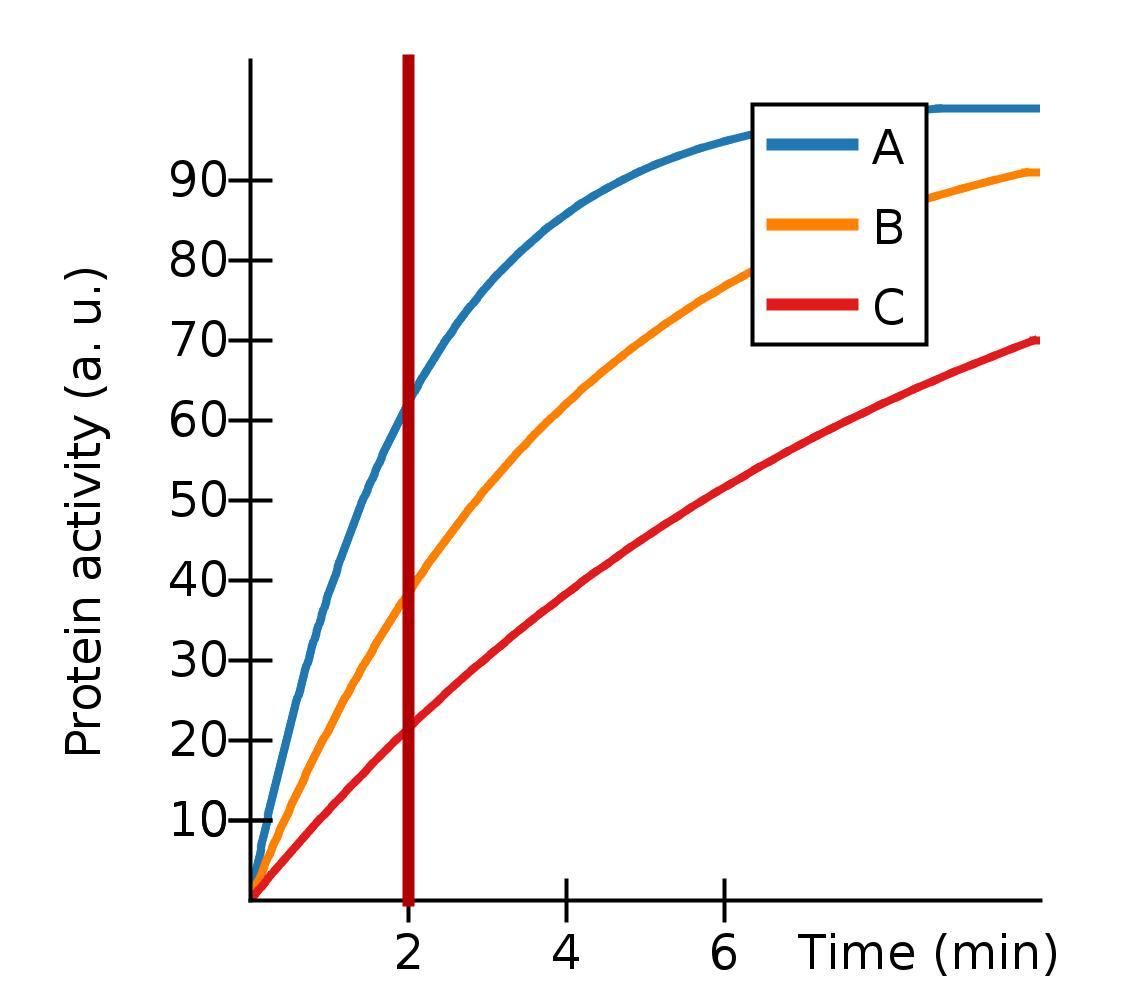
\includegraphics[scale=0.1]{images/starting_activity_graph}}
\newlength\graficoHeight
\setlength\graficoHeight{\heightof{\graficoStartingActivity}}
\def\scenarioDialog{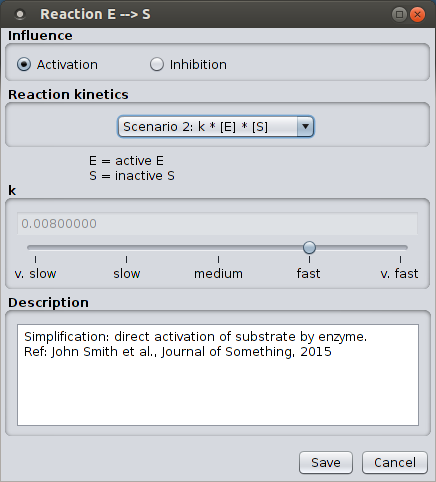
\includegraphics[scale=0.27]{images/scenario_parameter_dialog}}
\newlength\dialogHeight
\setlength\dialogHeight{\heightof{\scenarioDialog}}

\frame[t]{ \frametitle{Analysis of Networks with Interactive MOdelling}
  \begin{itemize}
    \item<1-> Interaction based \vspace{1ex}
    \item<1-> Discrete concentration/activity levels \vspace{1ex}
    \item<1-> Precise reactions $\Rightarrow$ abstract \emph{interactions}\only<2-3>{$$
\mbox{\it E} + \mbox{\it S} + \mbox{\it ATP} \rightleftarrows \mbox{\it ES} + \mbox{\it ATP} \rightarrow \mbox{\it ES}^{\mbox{\scriptsize \it P}} + \mbox{\it ADP} \rightleftarrows \mbox{\it E} + \mbox{\it S}^{\mbox{\scriptsize\it P}} + \mbox{\it ADP}
$$
(with $\mbox{\it S} + \mbox{\it S}^{\mbox{\scriptsize\it P}} = \mbox{constant}$ and $\mbox{\it ATP} + \mbox{\it ADP} = \mbox{constant}$)\\
\only<3-3>{\begin{center}\Large$\Downarrow$\end{center}\vspace{-1ex}\ \\
\begin{center}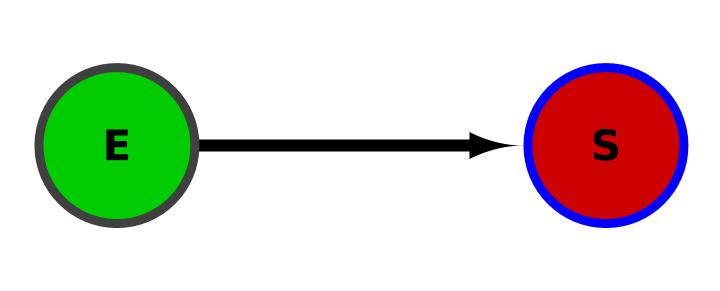
\includegraphics[width=0.3\textwidth]{images/interaction_E_S}\end{center}}} \vspace{1ex}
    \item<4-> Simplified scenarios for rate computation\\\hspace{-0.8cm}\begin{minipage}[c][\dialogHeight]{0.4\textwidth}\begin{center}\scenarioDialog\end{center}\end{minipage} \begin{minipage}[c][\dialogHeight]{0.3\textwidth}\begin{center}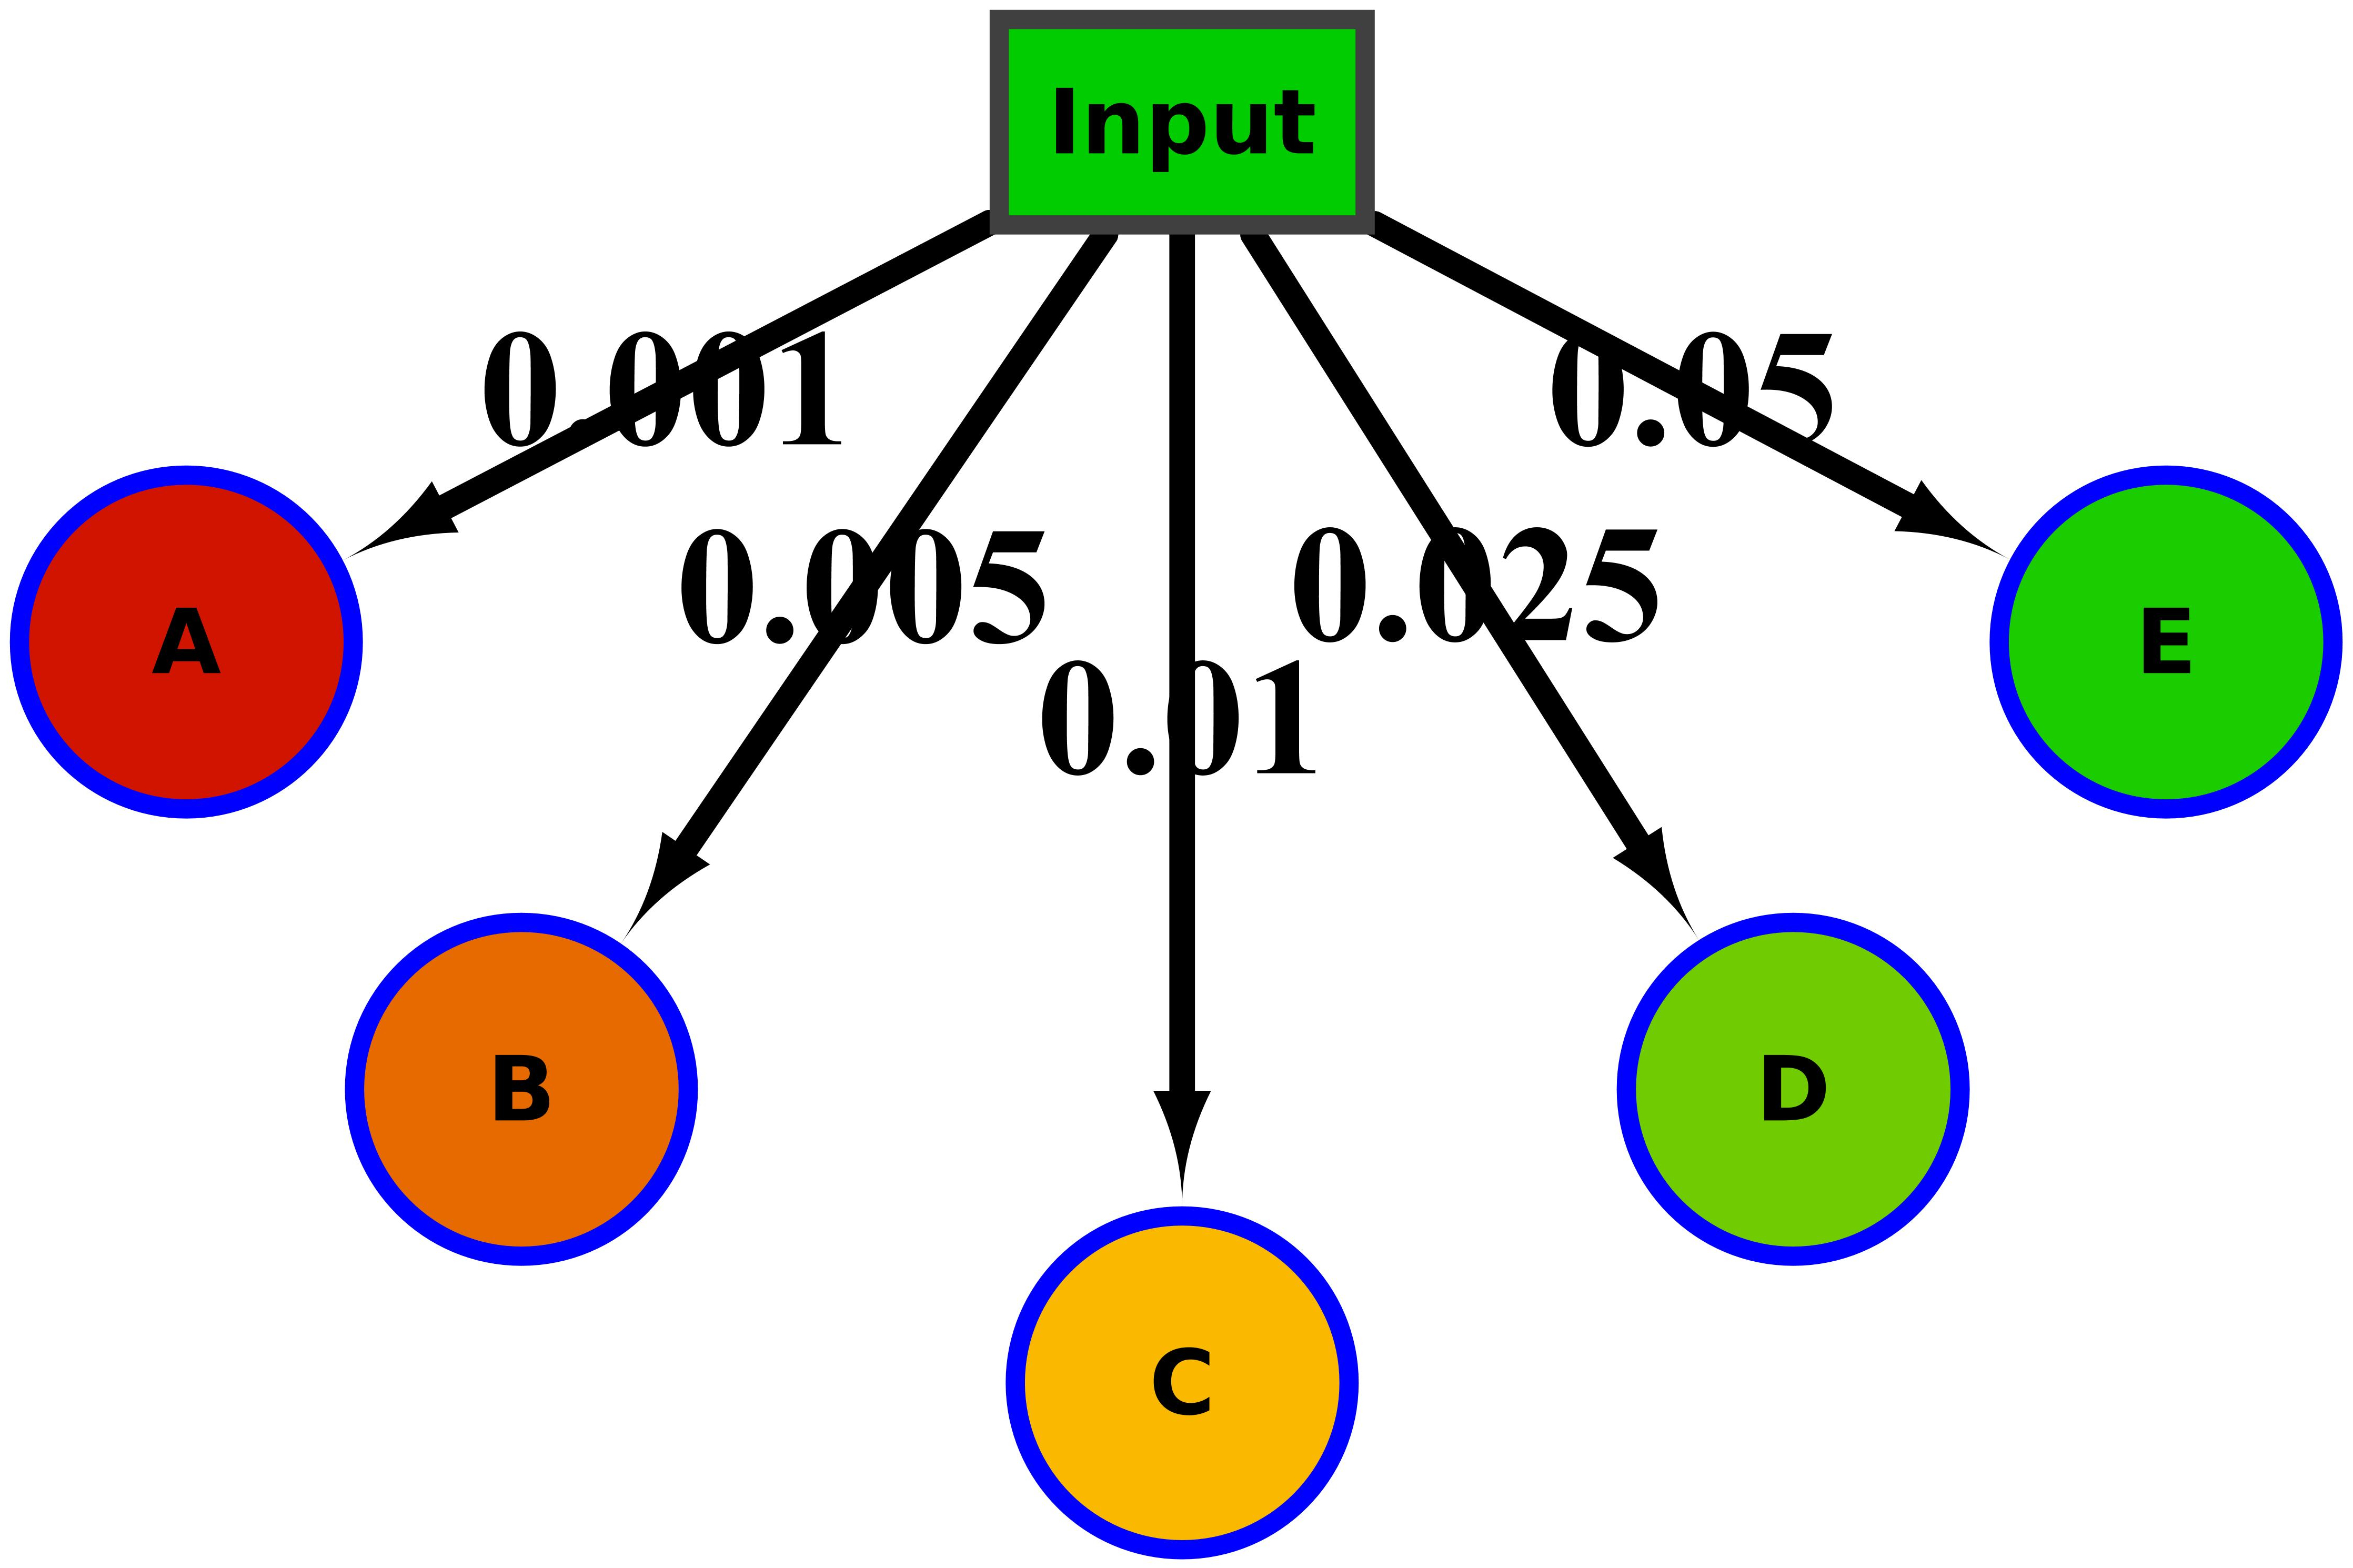
\includegraphics[scale=0.015]{images/parameter_network}\vspace{2ex}\\\pgfuseimage{activity-legend}\end{center}\end{minipage} \begin{minipage}[c][\dialogHeight]{0.2\textwidth}\begin{center}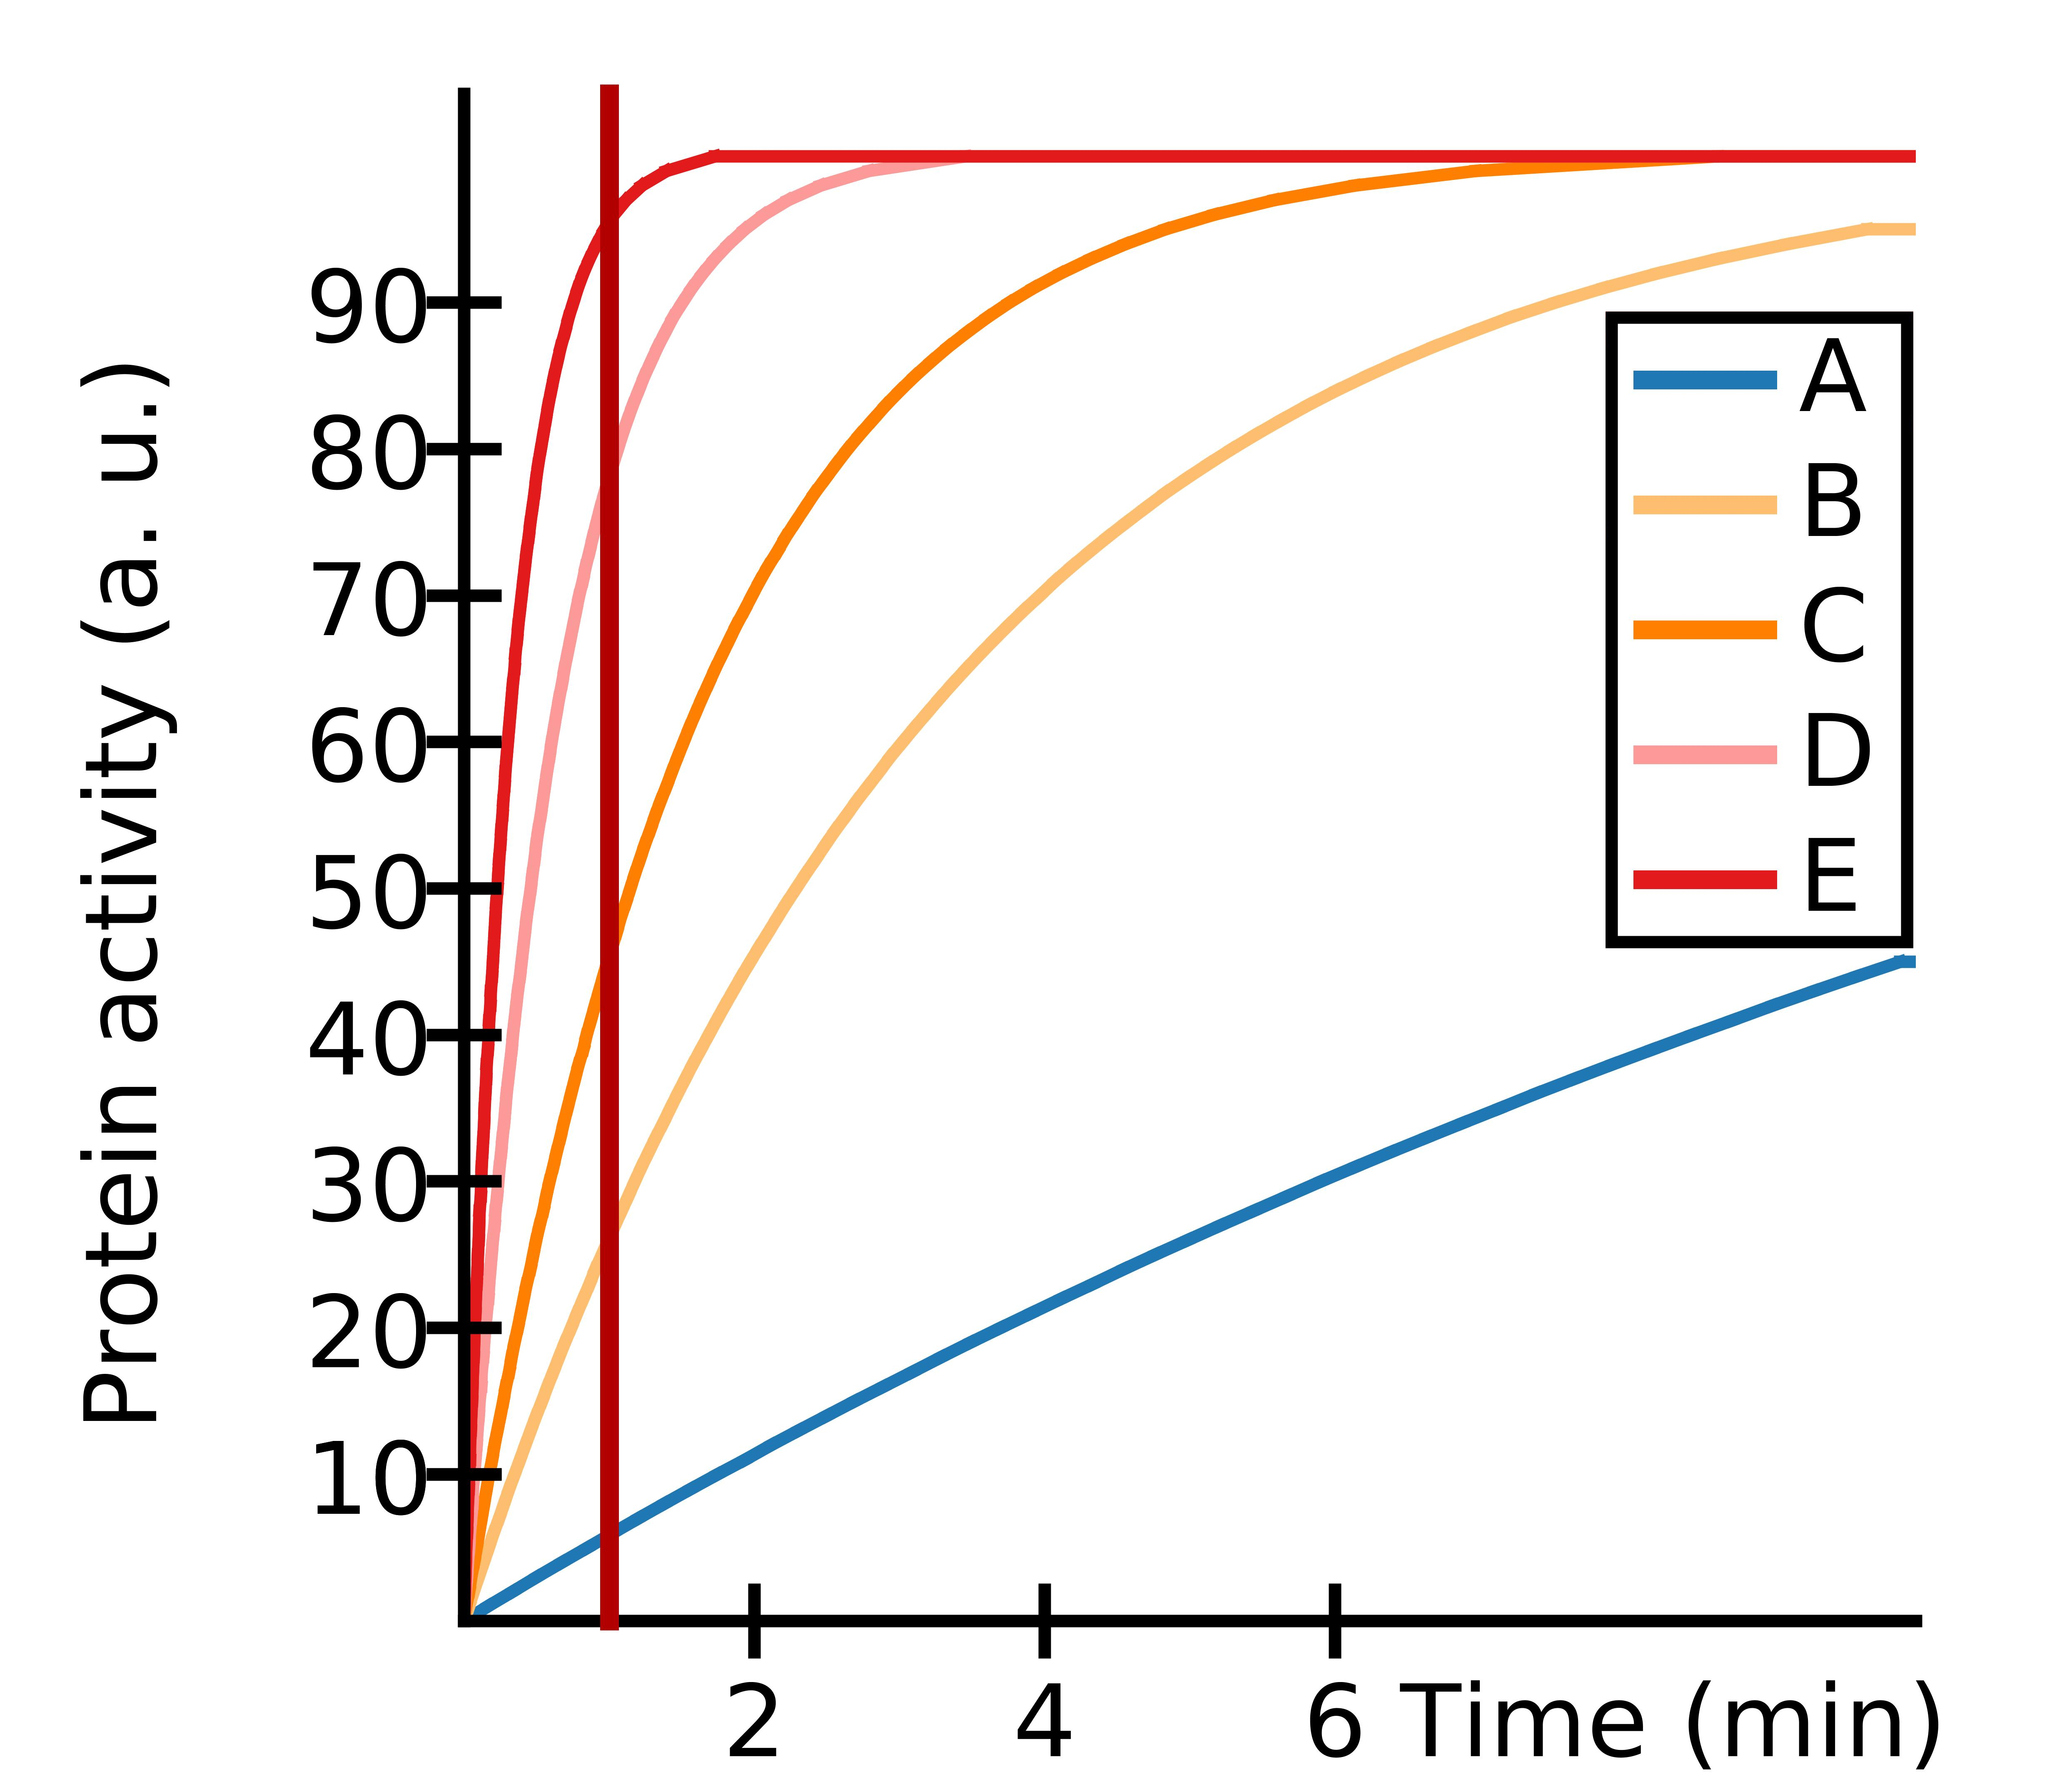
\includegraphics[scale=0.02]{images/parameter_graph}\end{center}\end{minipage} \vspace{1ex}
%\only<5-5>{\begin{minipage}[c][\dialogHeight]{0.3\textwidth}\begin{center}\includegraphics[scale=0.015]{images/scenario1-2_network}\vspace{2ex}\\\pgfuseimage{activity-legend}\end{center}\end{minipage} \begin{minipage}[c][\dialogHeight]{0.2\textwidth}\begin{center}\includegraphics[scale=0.02]{images/scenario1-2_graph}\end{center}\end{minipage}}
    %\item<6-> Reactant activity levels determine interaction rates\only<8->{\begin{center}\begin{minipage}[c][\graficoHeight]{0.15\textwidth}\begin{center}\includegraphics[scale=0.35]{images/activity_legend_vertical}\end{center}\end{minipage}\quad\begin{minipage}[c][\graficoHeight]{0.3\textwidth}\begin{center}\includegraphics[scale=0.065]{images/starting_activity_network}\end{center}\end{minipage}\qquad\begin{minipage}[c][\graficoHeight]{0.35\textwidth}\begin{center}\graficoStartingActivity\end{center}\end{minipage}\end{center}} \vspace{1ex}
  \end{itemize}
}


\frame{ \frametitle{Timed Automata model}
  \begin{center}
    \pgfuseimage{ta-reactant-centered}
  \end{center}
}



\frame{\frametitle{ANIMO workflow}
\only<1-1>{Start from static network topology\\\begin{center}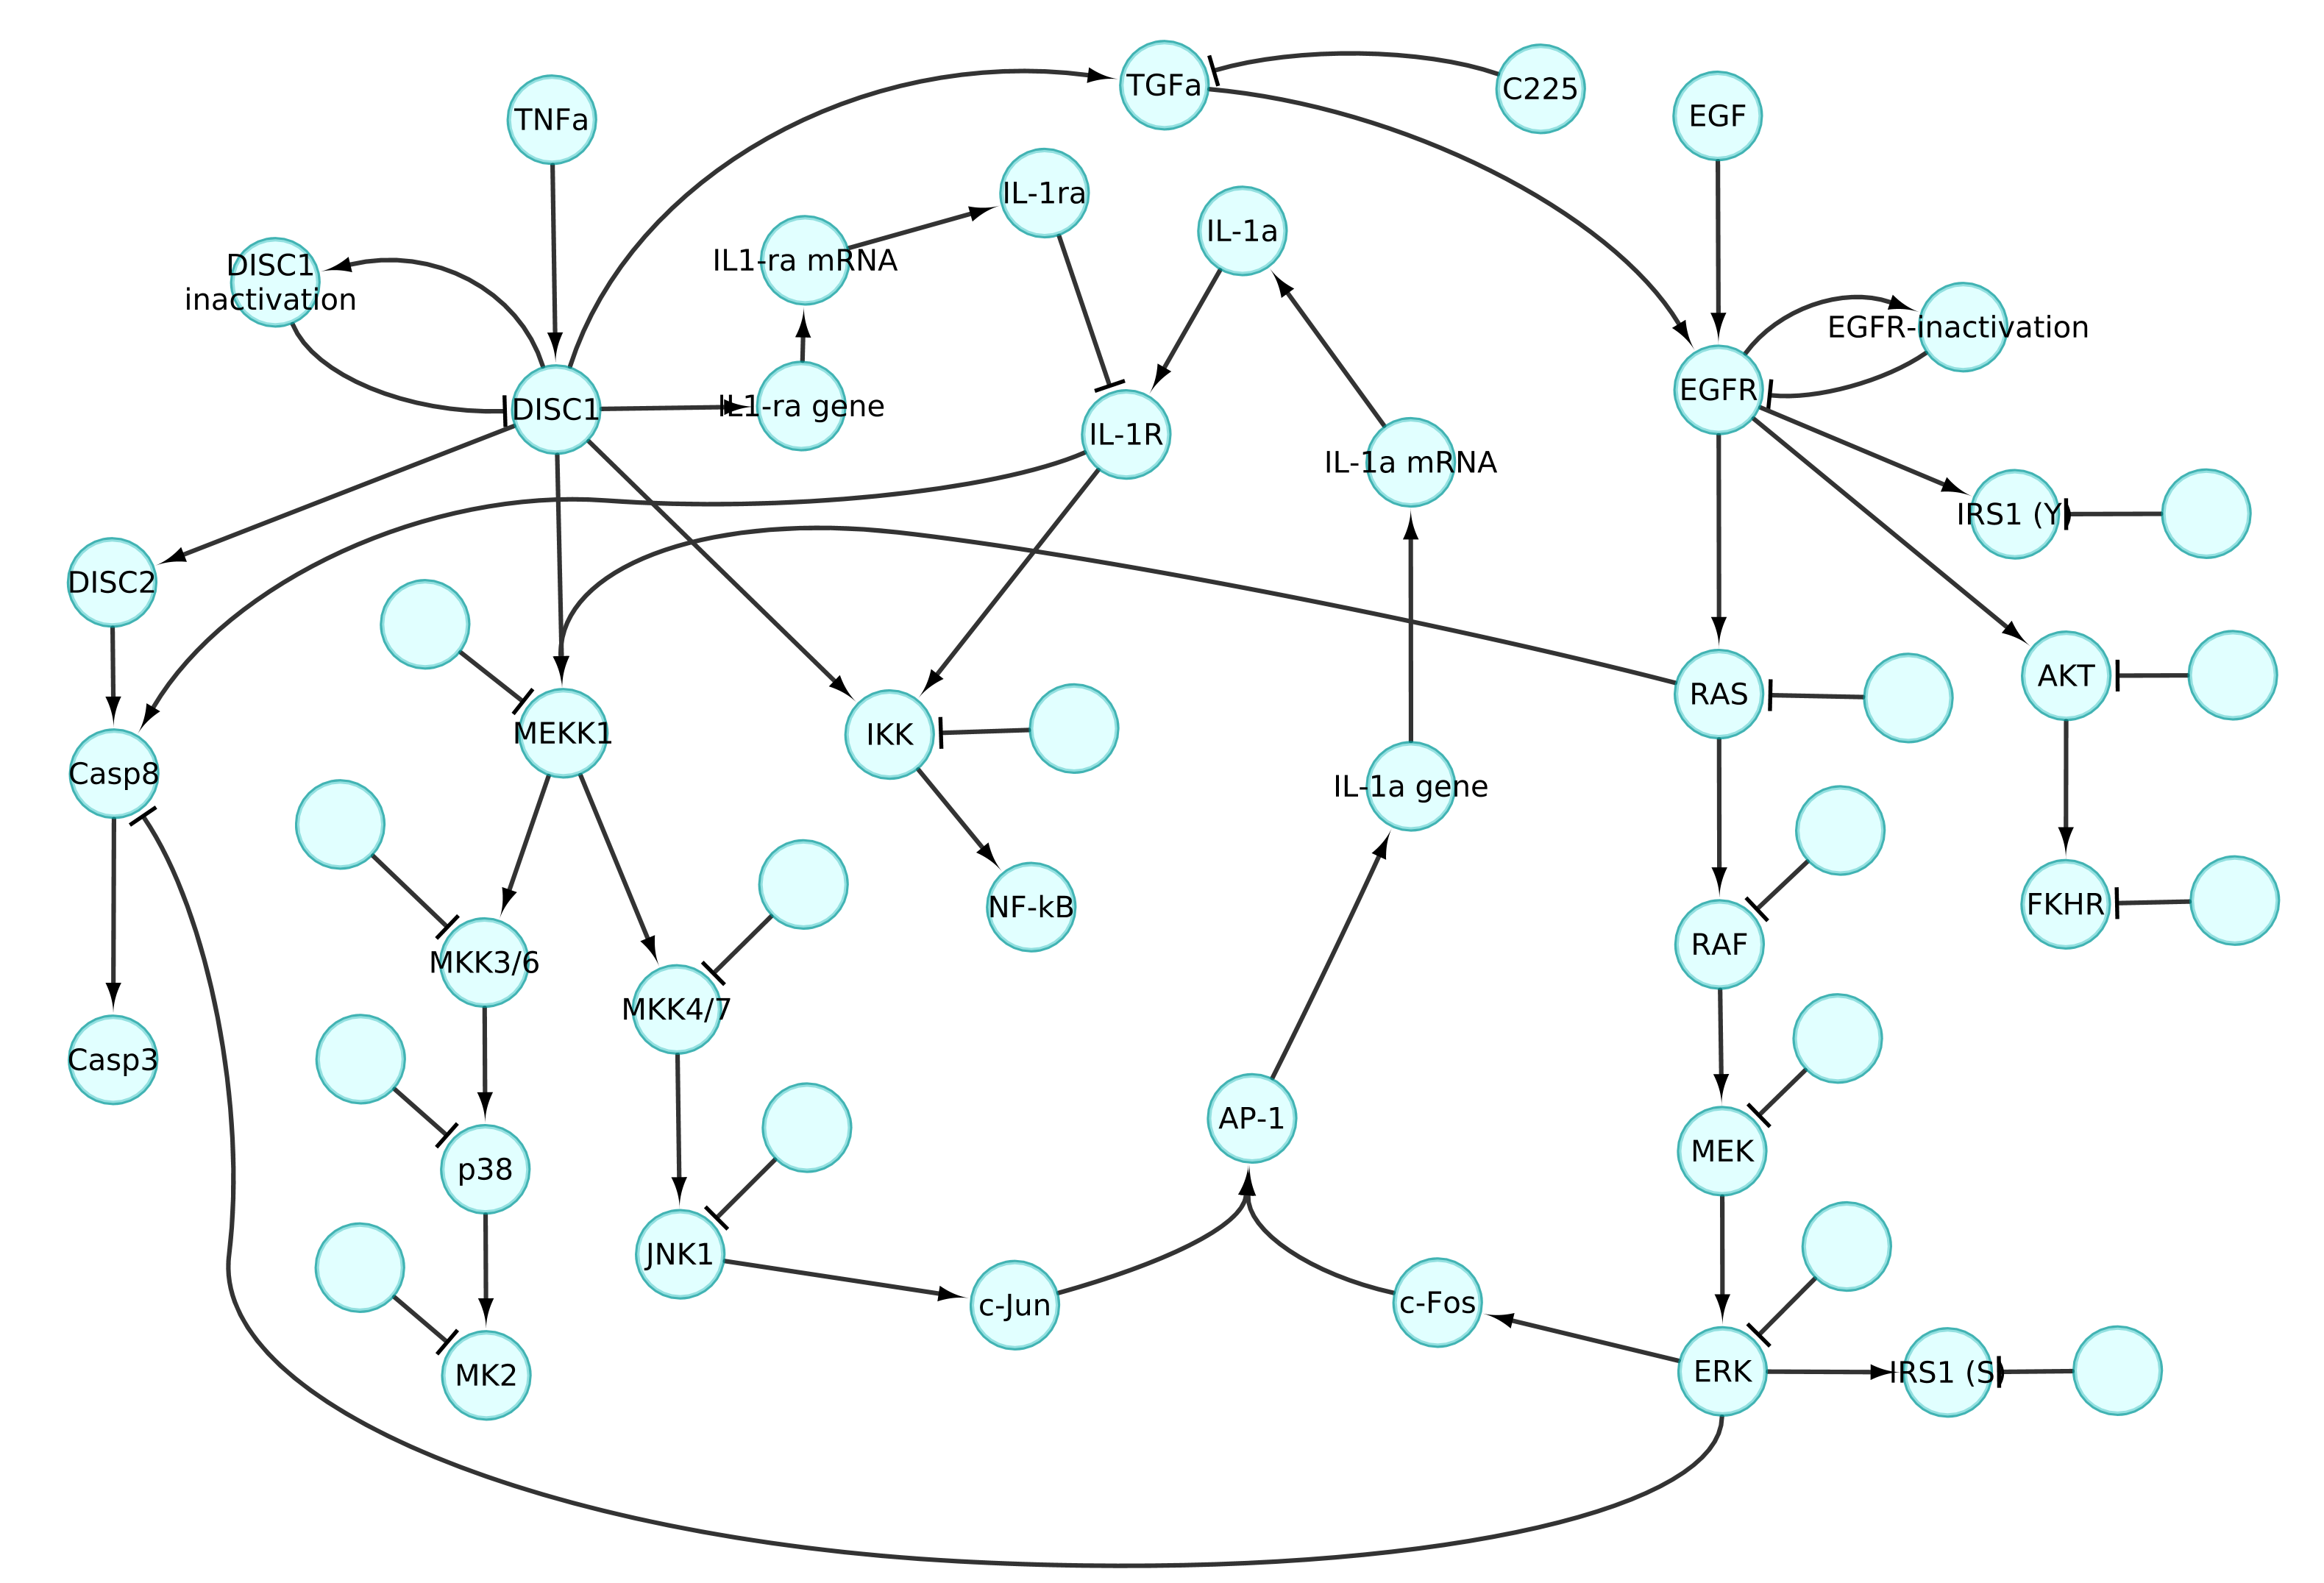
\includegraphics[width=0.9\textwidth]{images/rete_iniziale}\end{center}}
\only<2-2>{Add kinetics and choose initial activities\\\begin{center}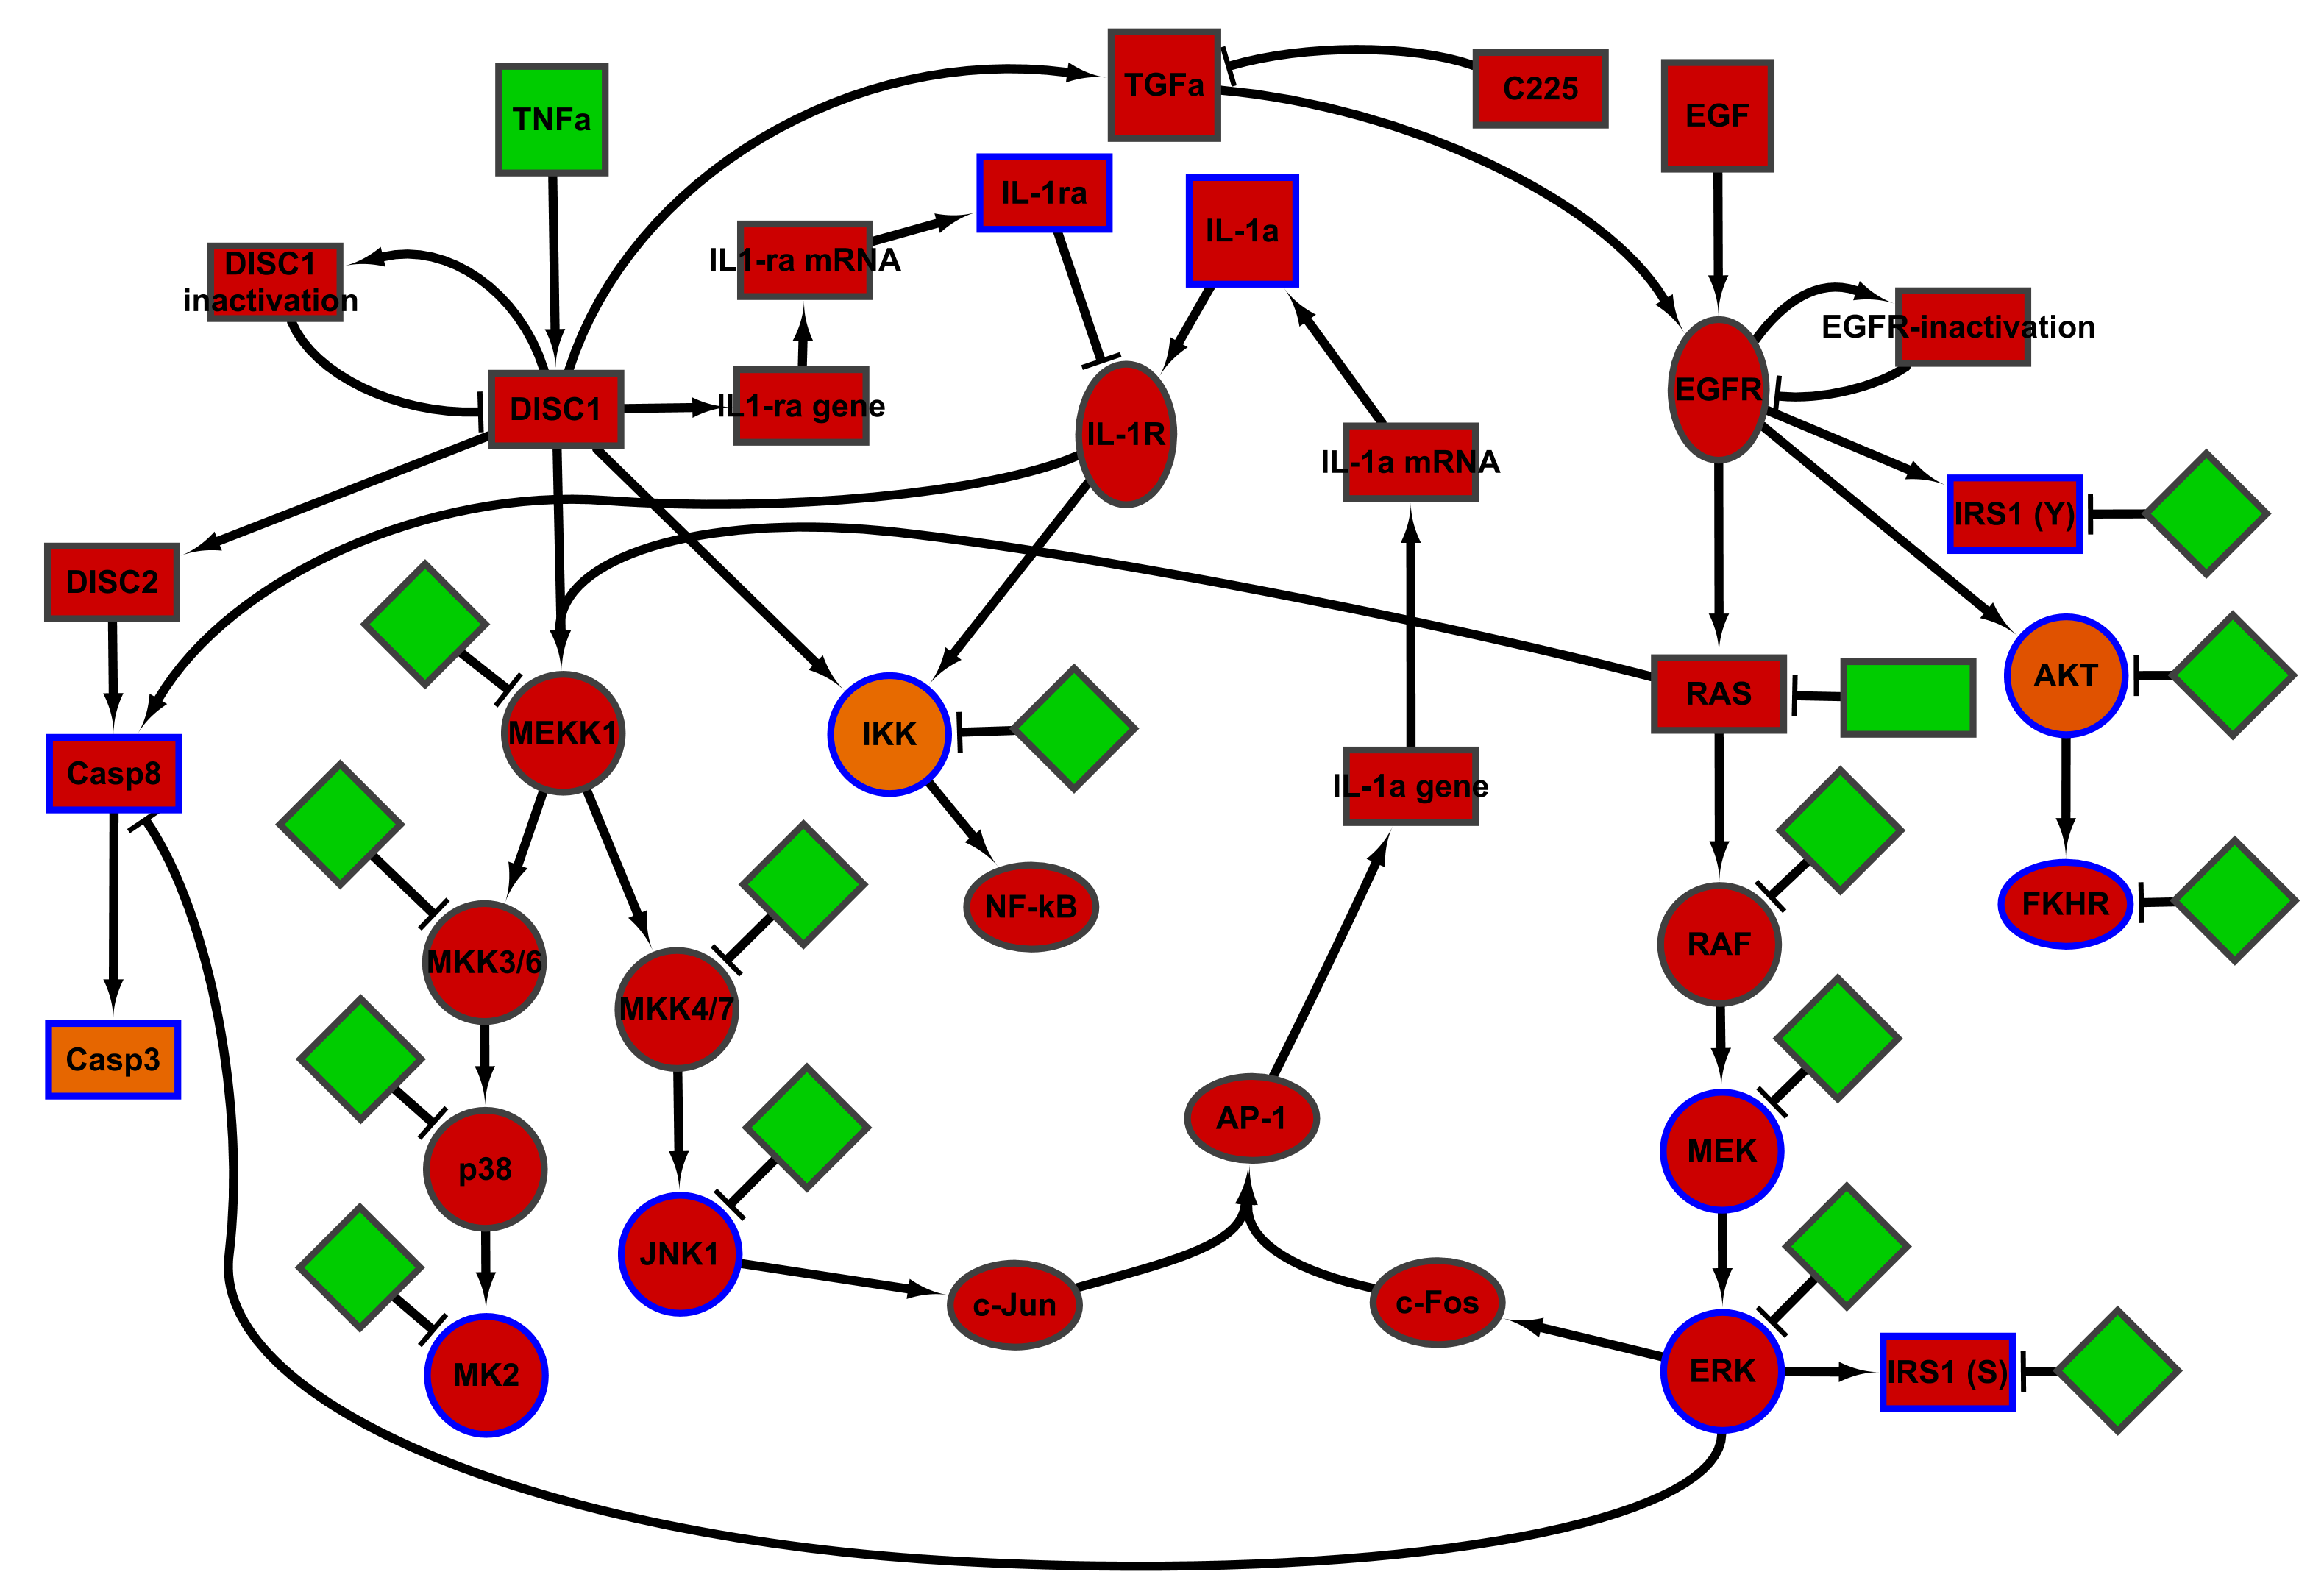
\includegraphics[width=0.9\textwidth]{images/rete_con_valori}\end{center}}
\only<3-5>{Inspect system evolution on the fly\vspace{-1.2ex}\\\begin{center}
\begin{tikzpicture}
  \draw <3-> node (1) at (0,0) {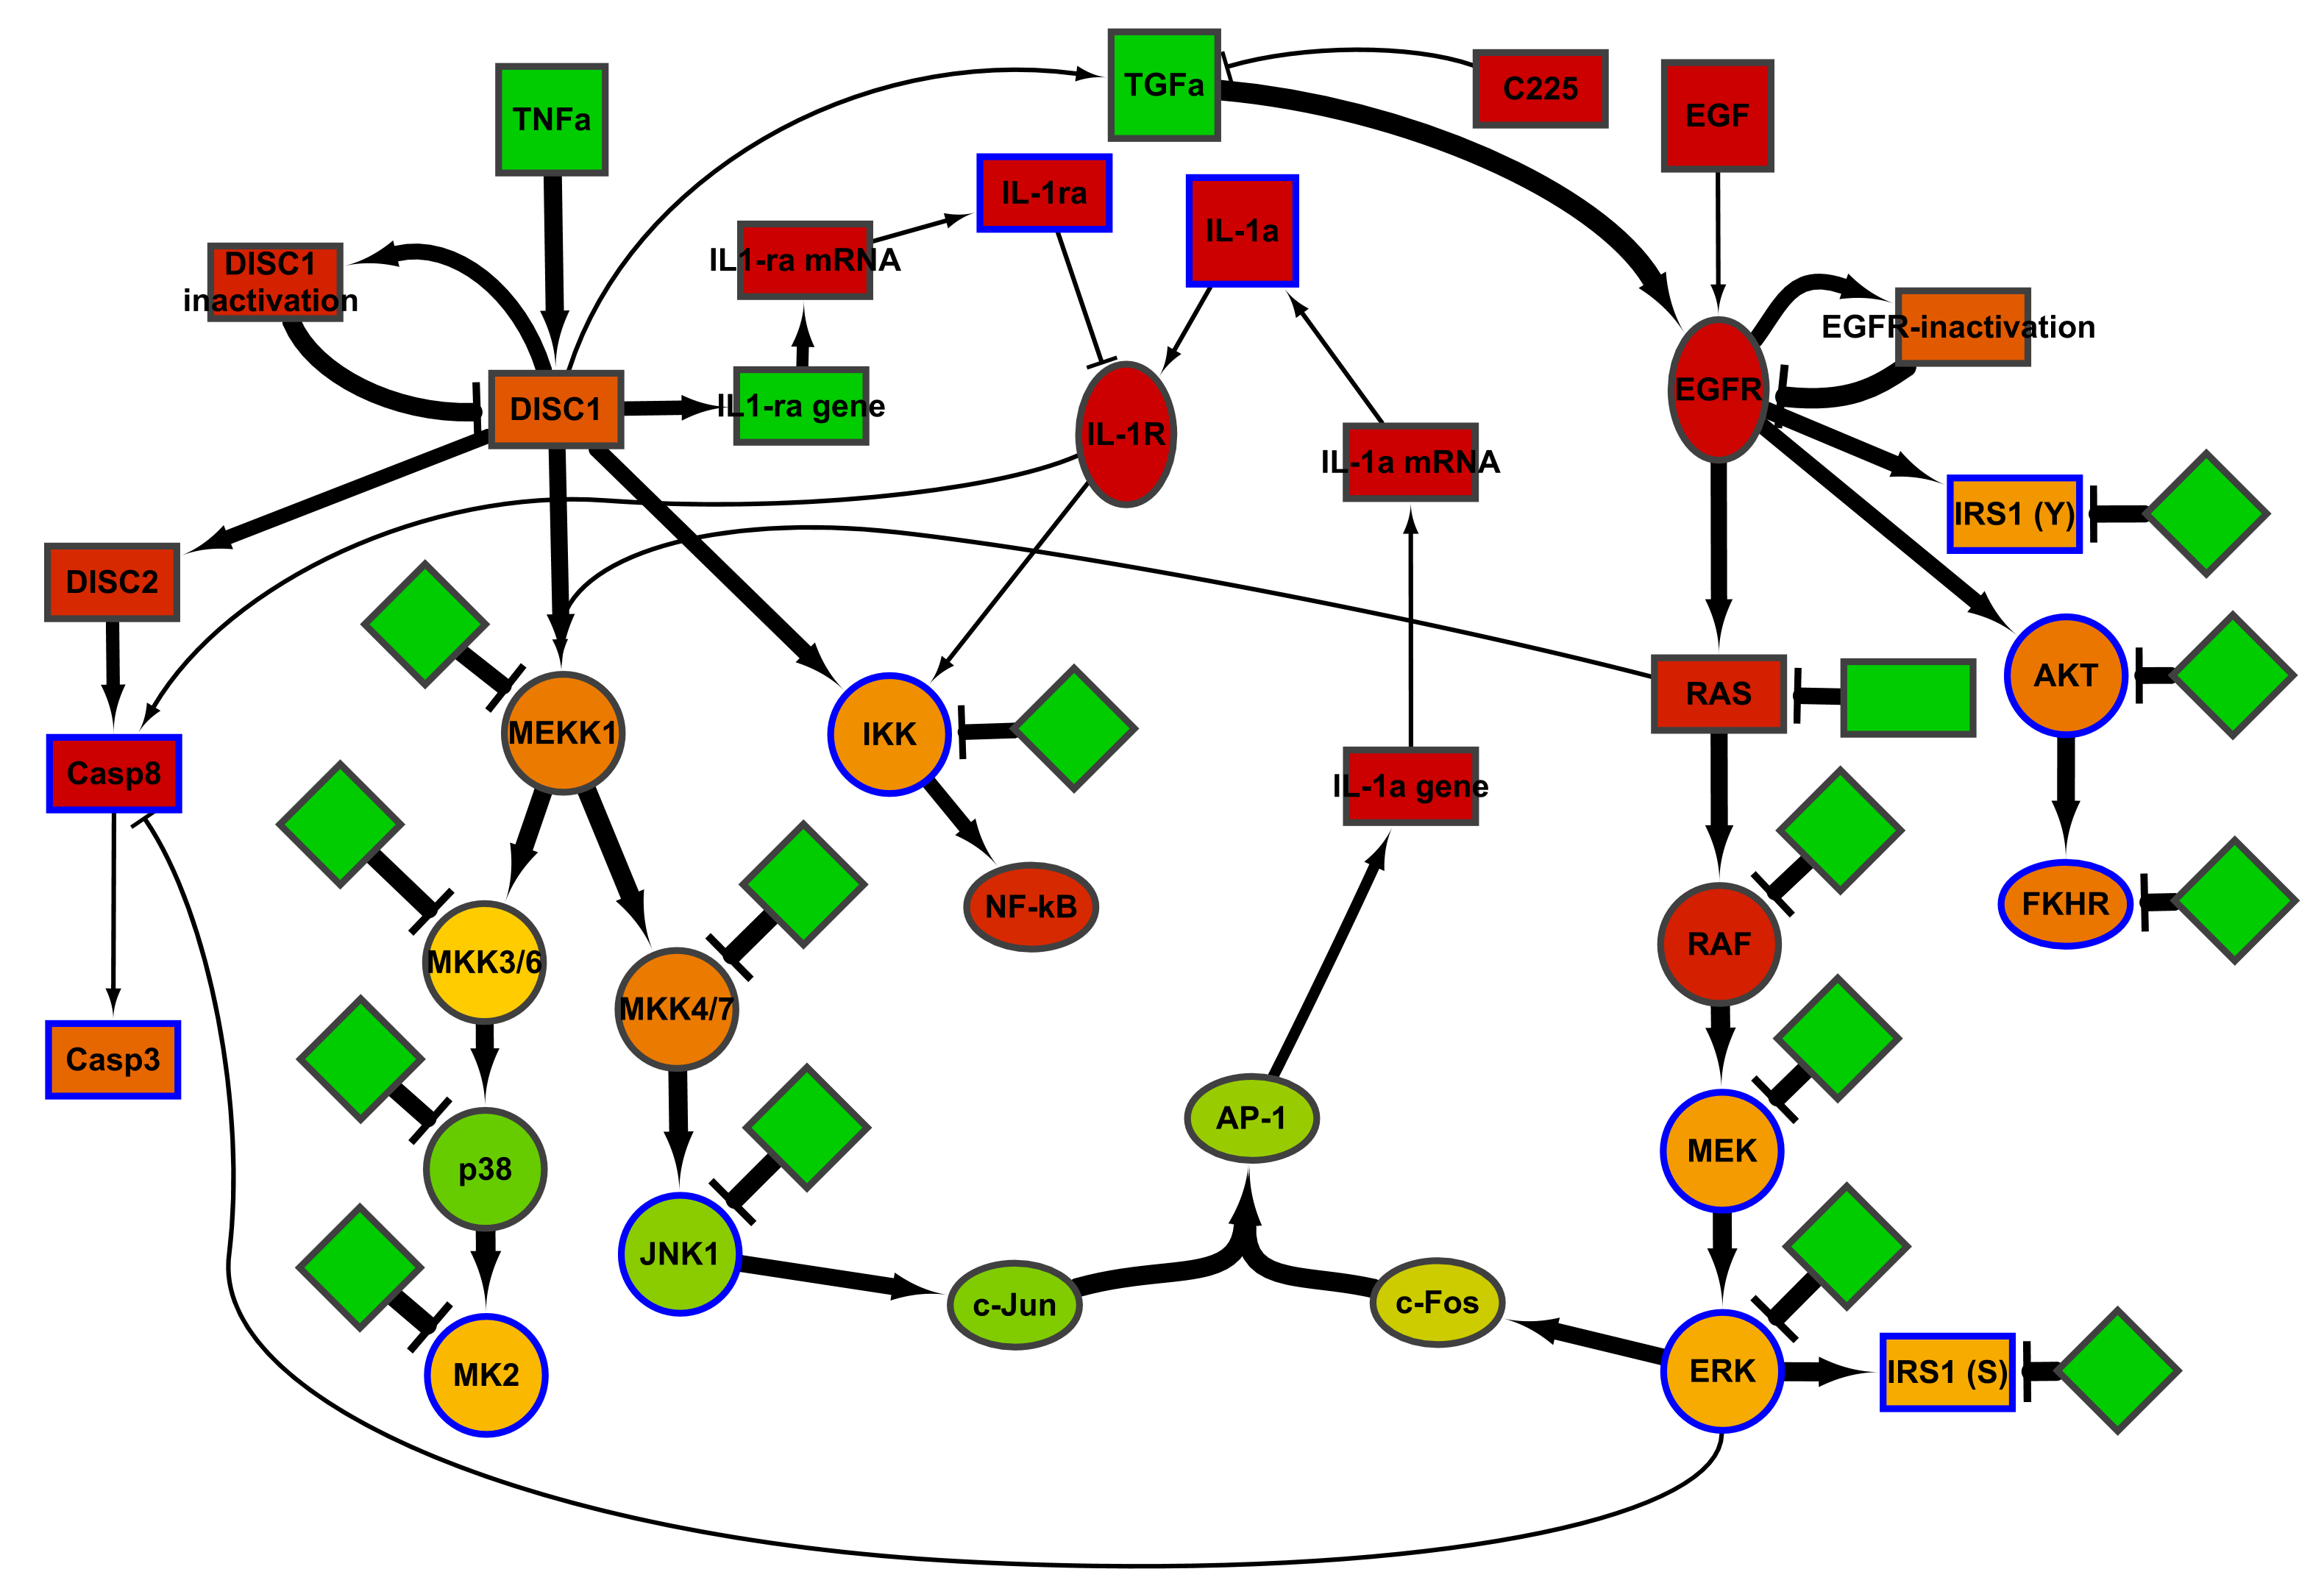
\includegraphics[width=0.9\textwidth]{images/rete_dinamica}};
  \draw <4-> node (2) at (2.1,1.3) {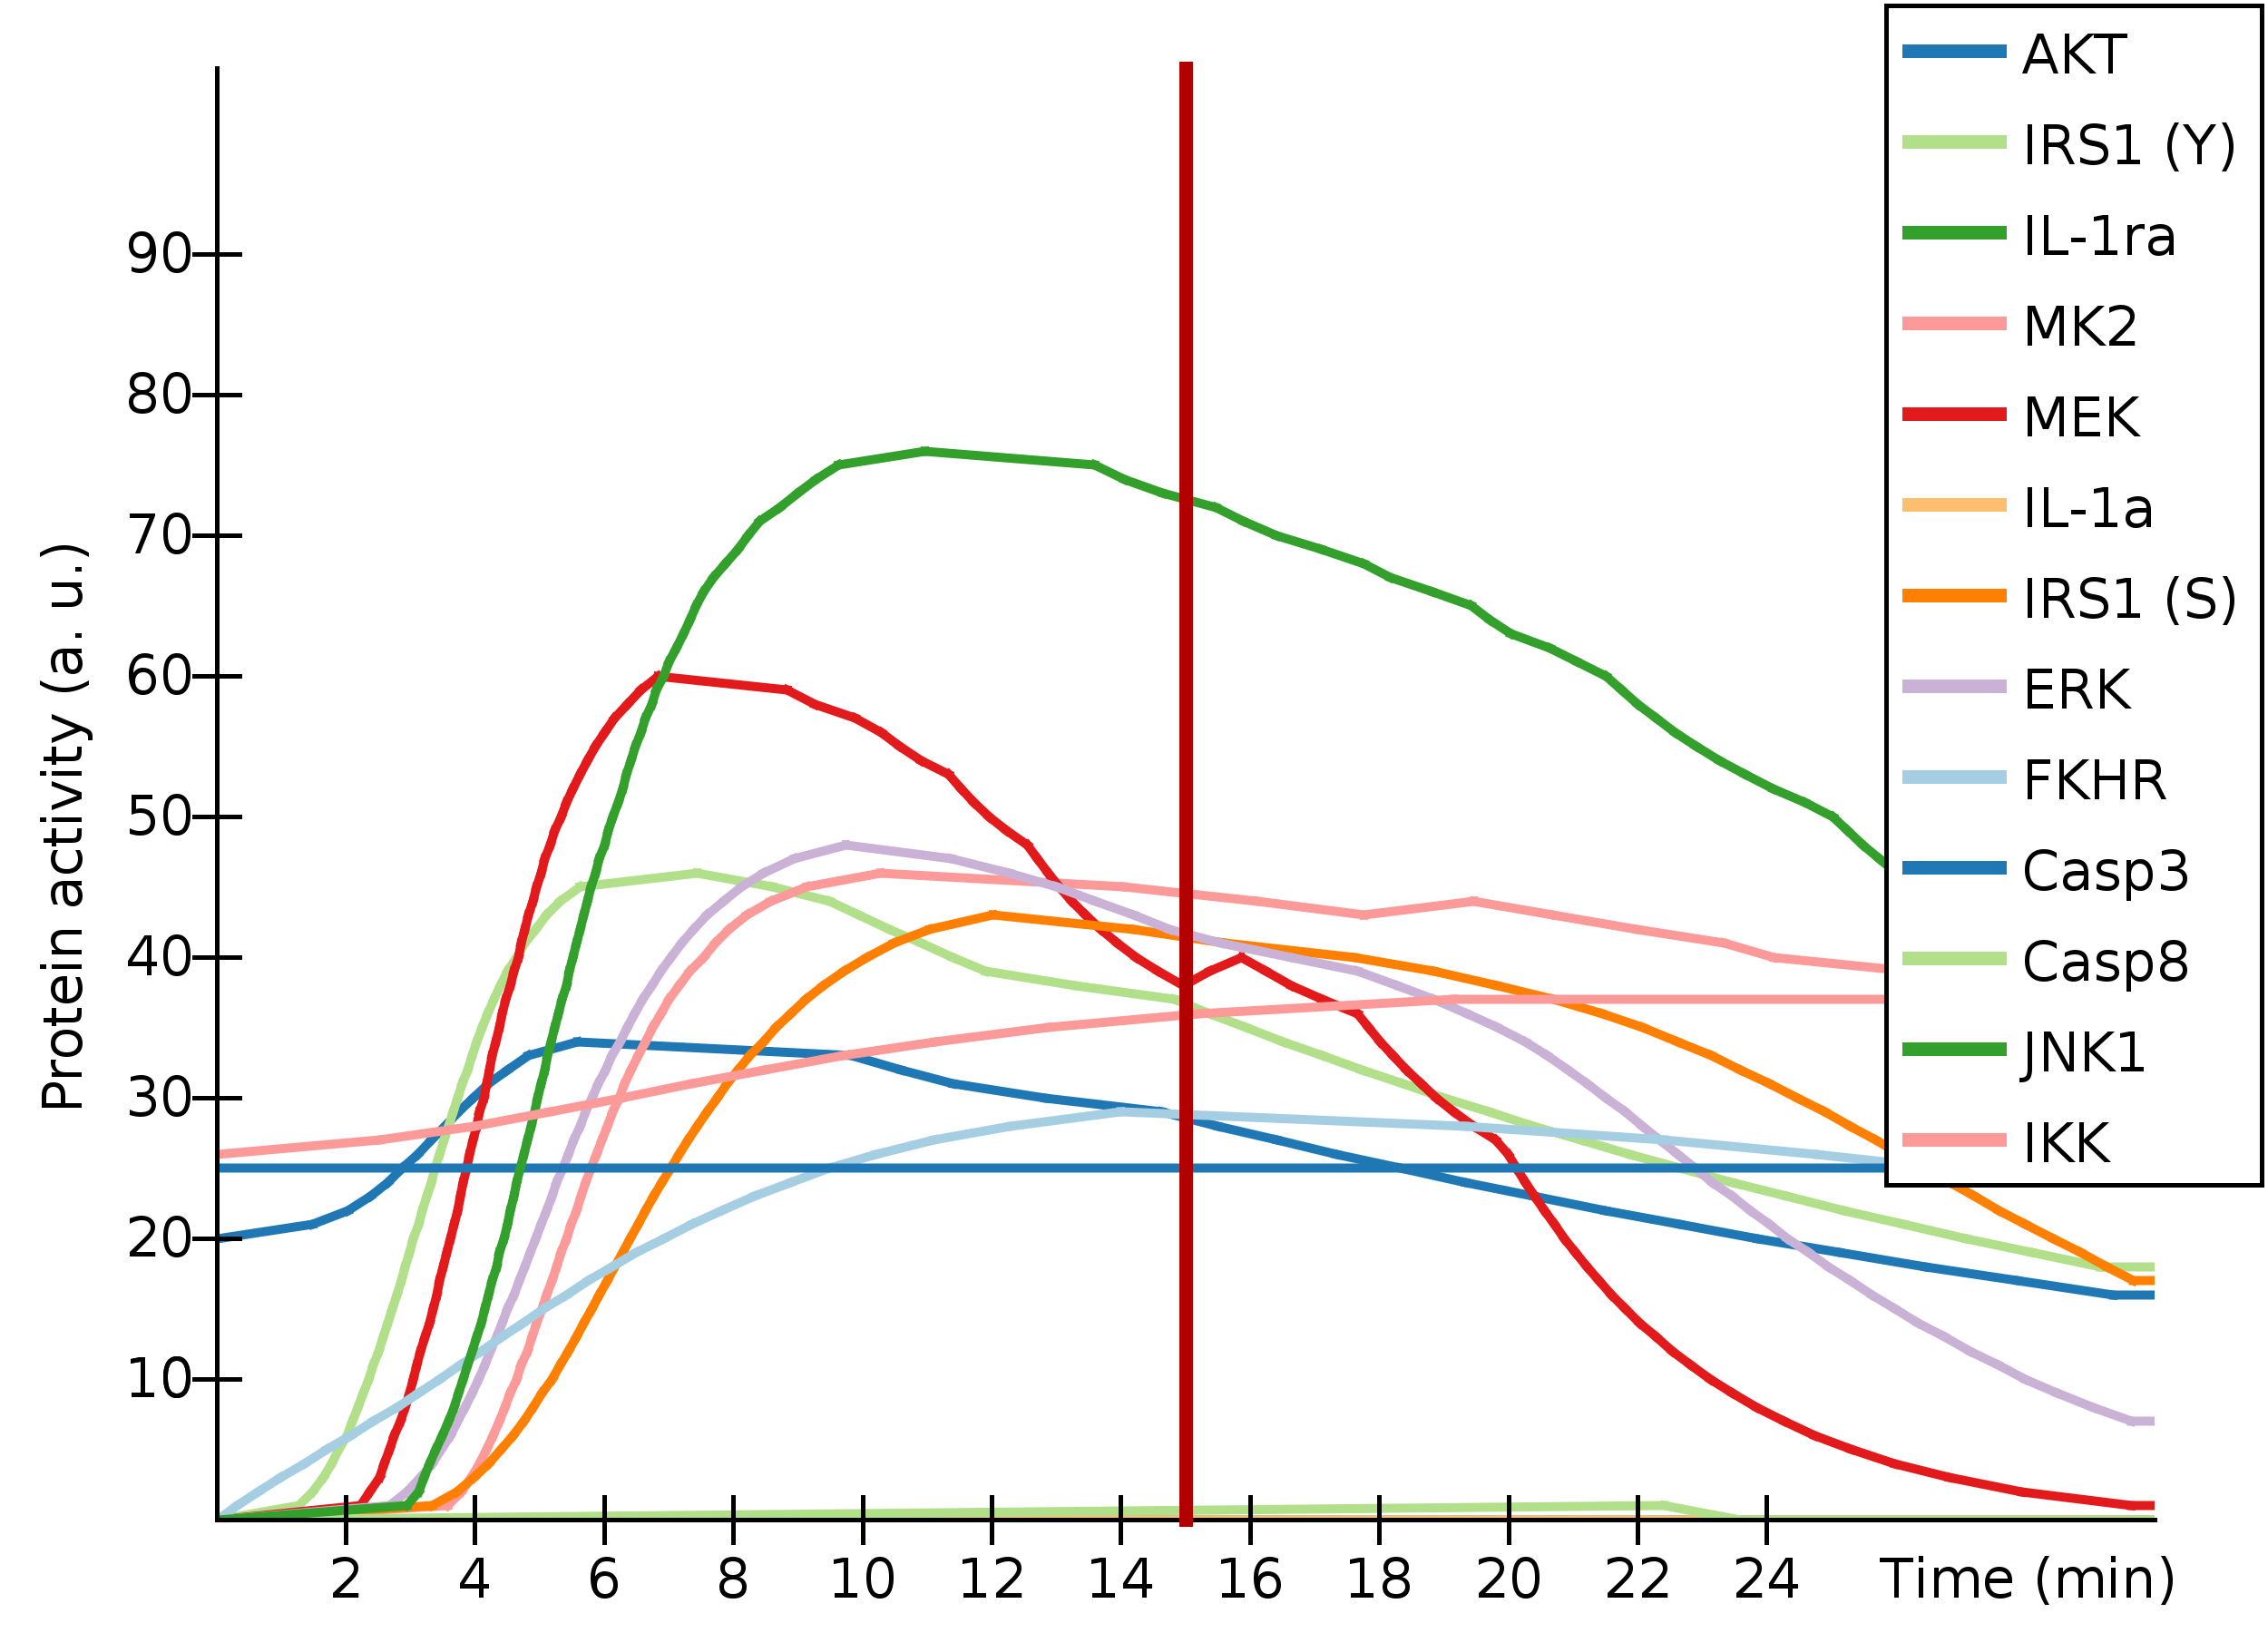
\includegraphics[width=0.5\textwidth]{images/grafico1}};
  \draw <5-> node (3) at (2.1,-1.4) {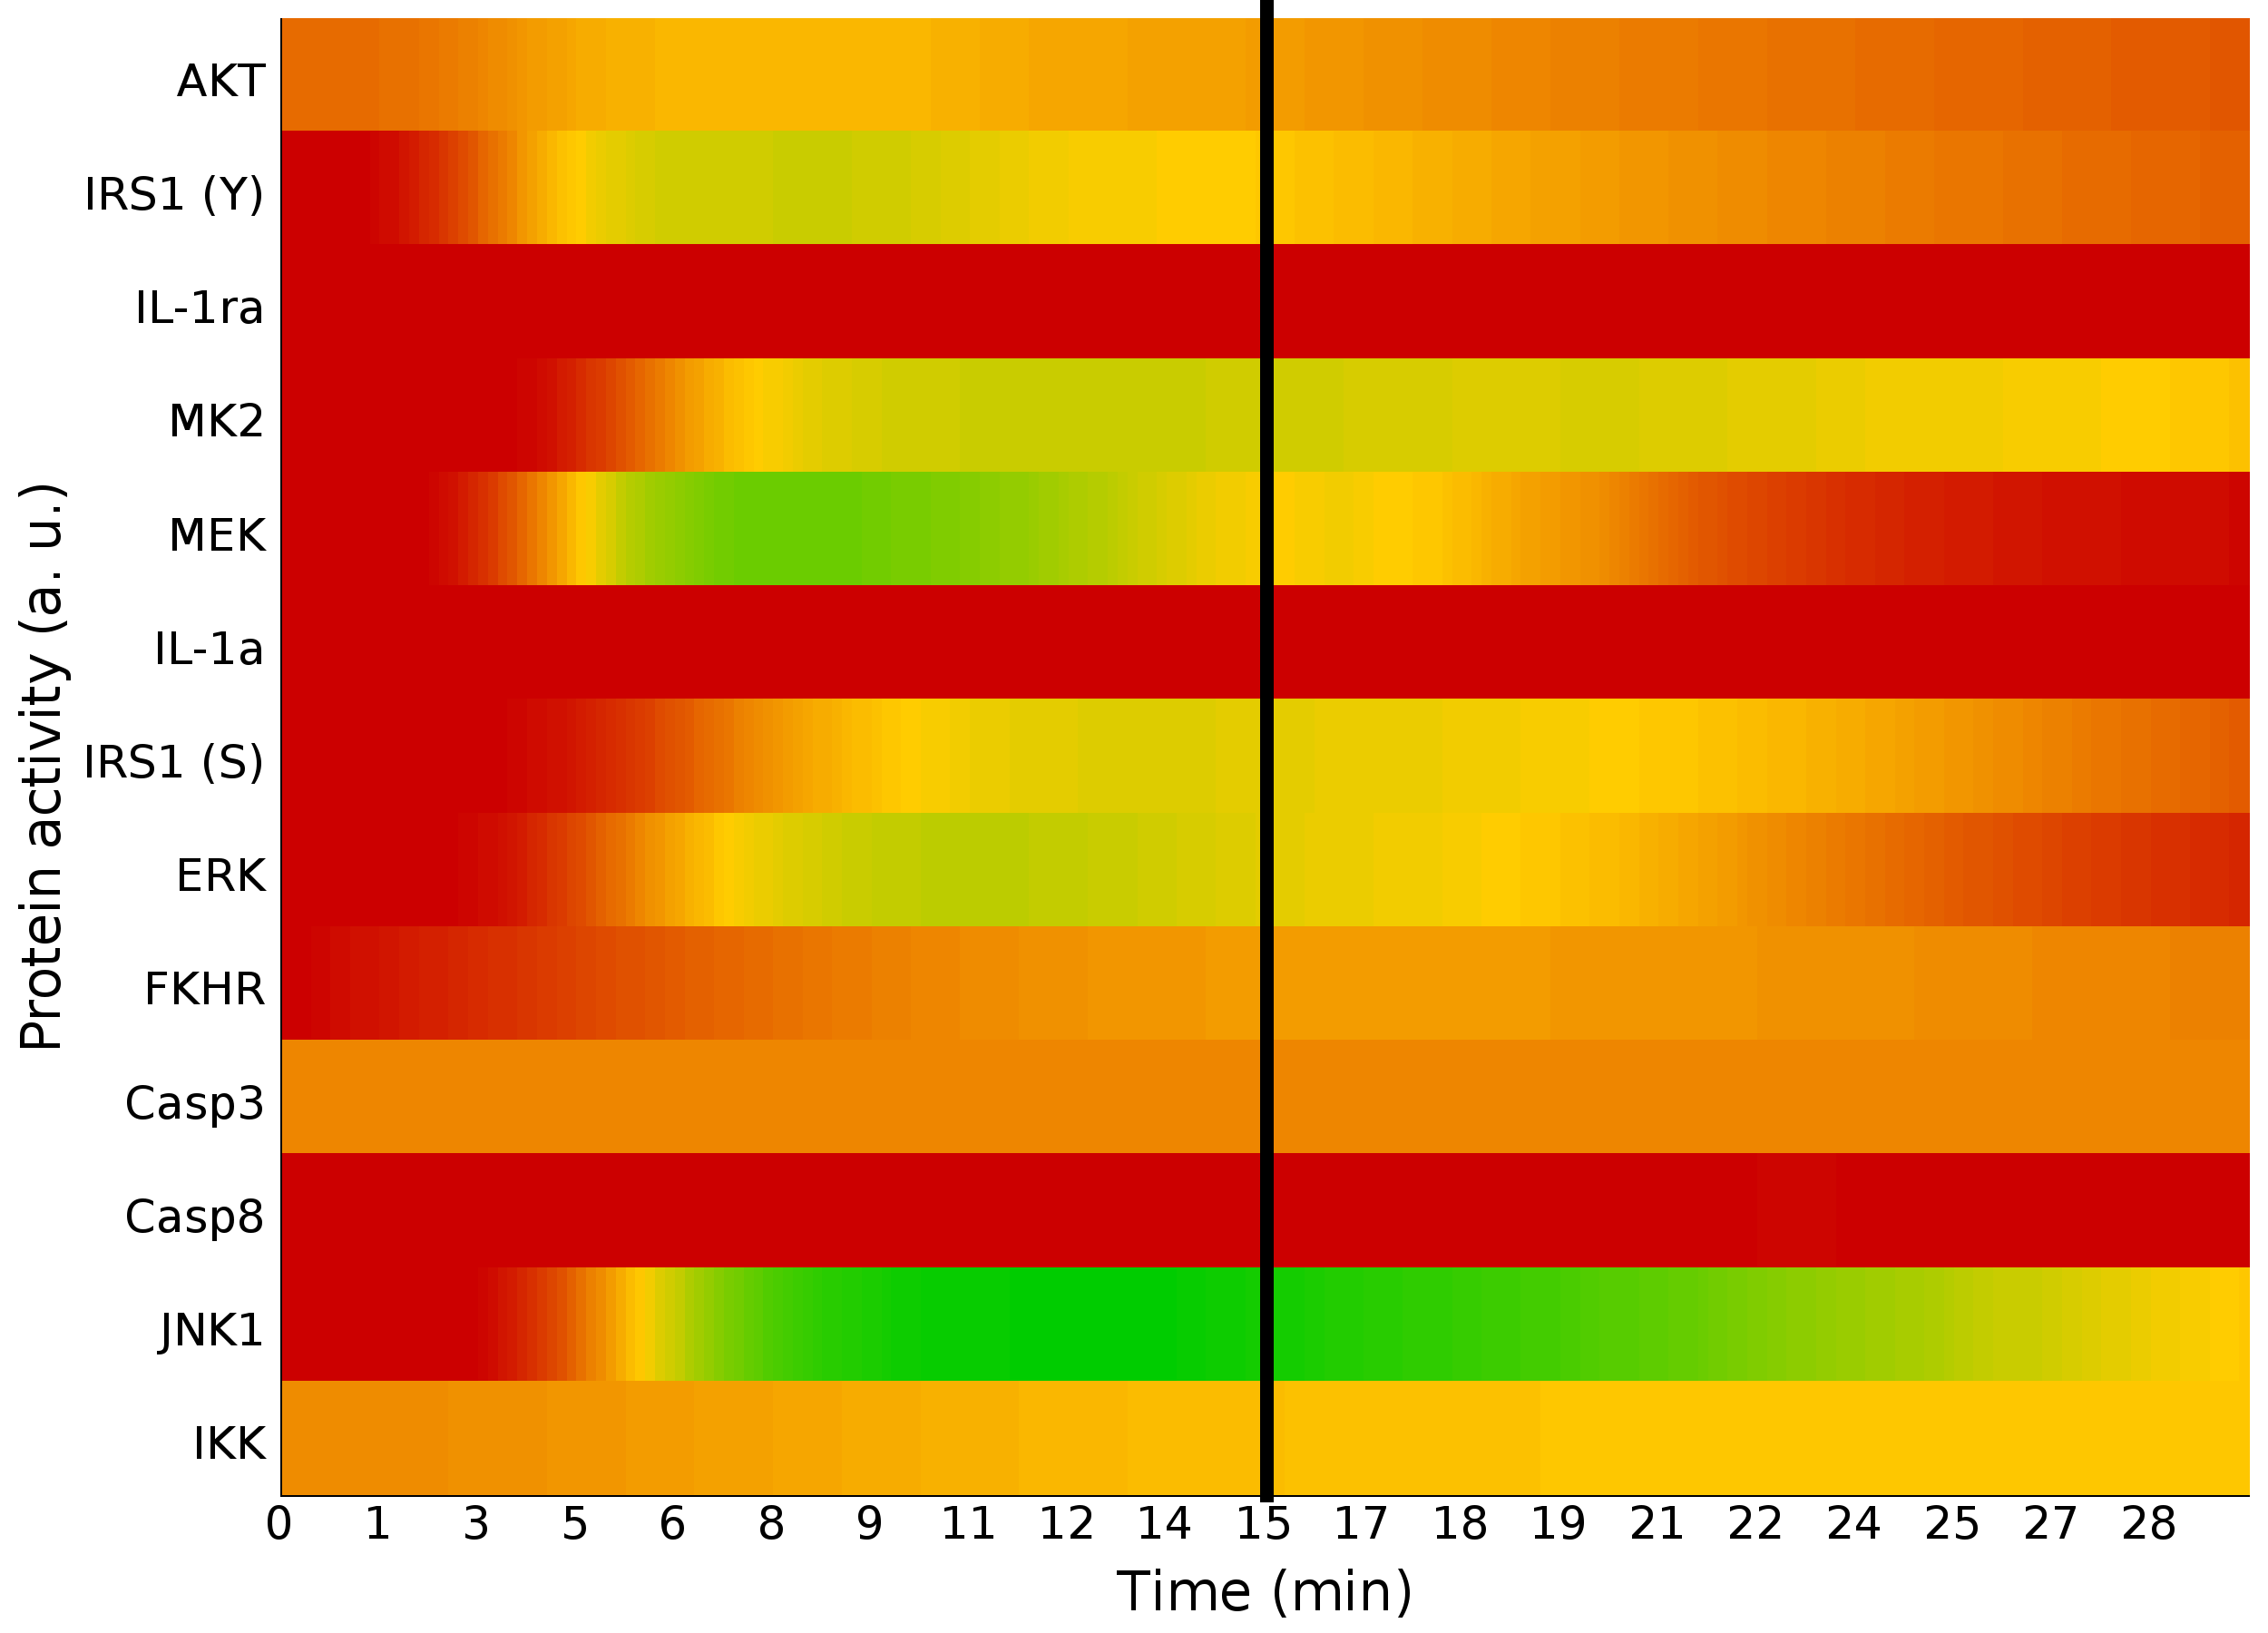
\includegraphics[width=0.5\textwidth]{images/grafico2}};
\end{tikzpicture}\end{center}}
}

\frame{\frametitle{Experimental data as reference}
\begin{center}
  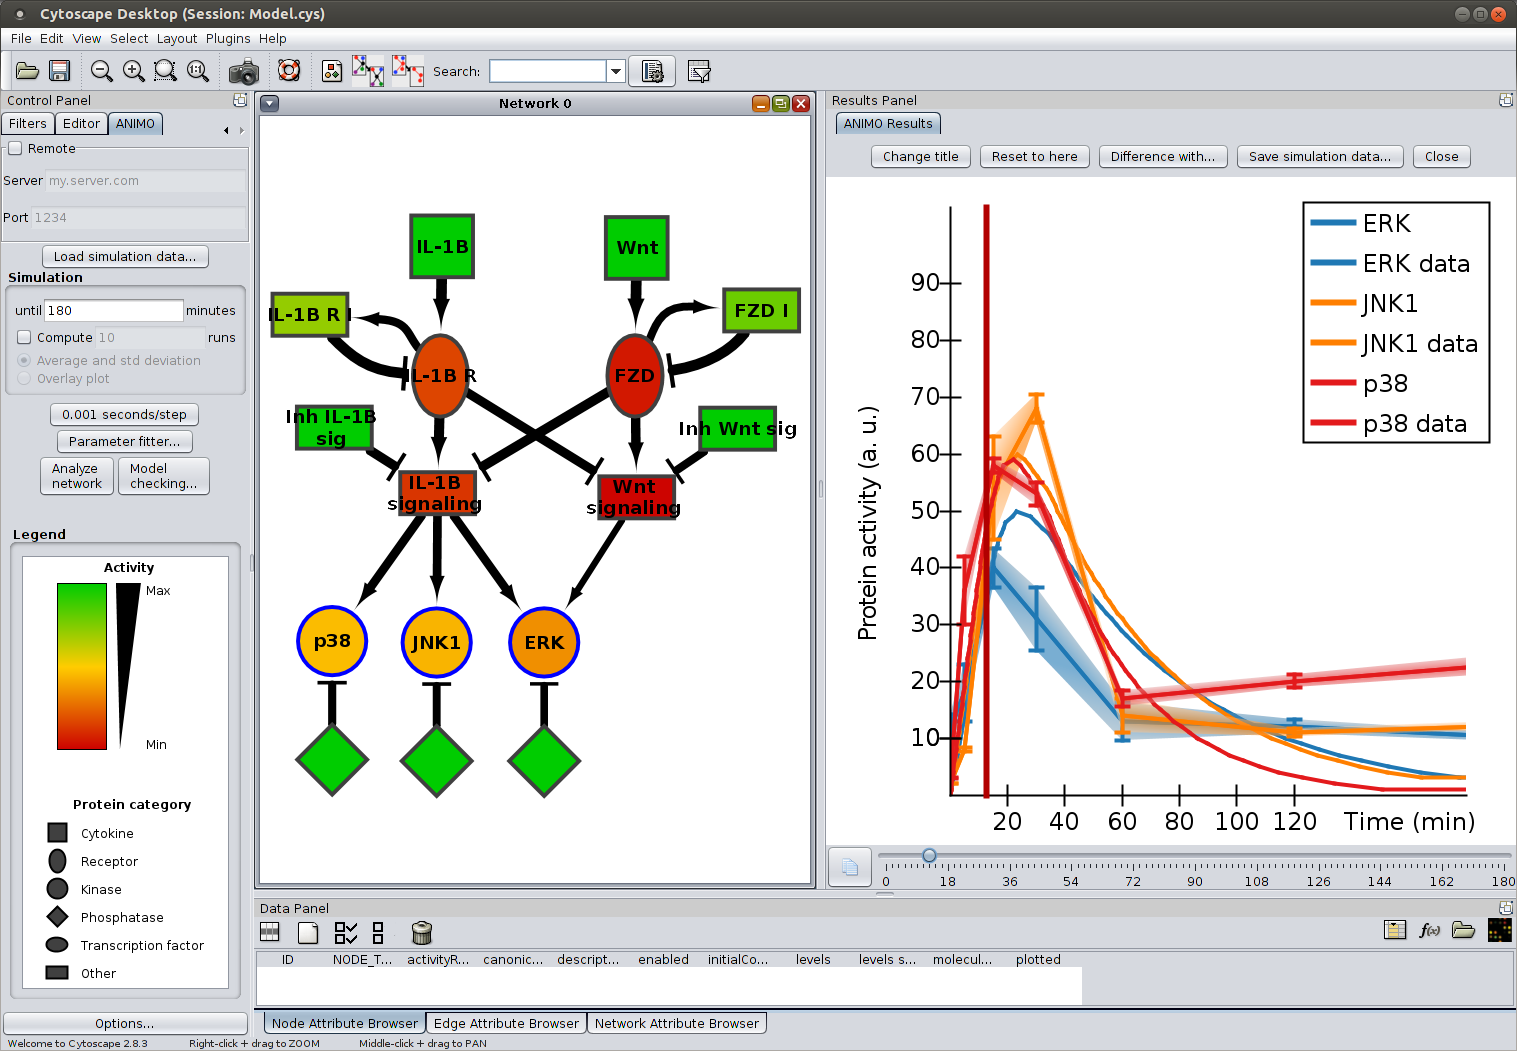
\includegraphics[width=0.8\textwidth]{images/chondrocyteModel}\ \\
Use data and model to improve knowledge, generate hypotheses.
\end{center}
}



\frame{\frametitle{All good and nice, but\dots}
{\Huge How to find the parameters?}\\ \ \\
\begin{itemize}
  \item<2-> ANIMO models are centered around the topology more than the parameters
  \item<3-> ANIMO requires less parameters than ODEs
  \item<4-> 
\end{itemize}
but we still need to estimate them
}


\frame{\frametitle{ANIMO live demo}
\begin{center}
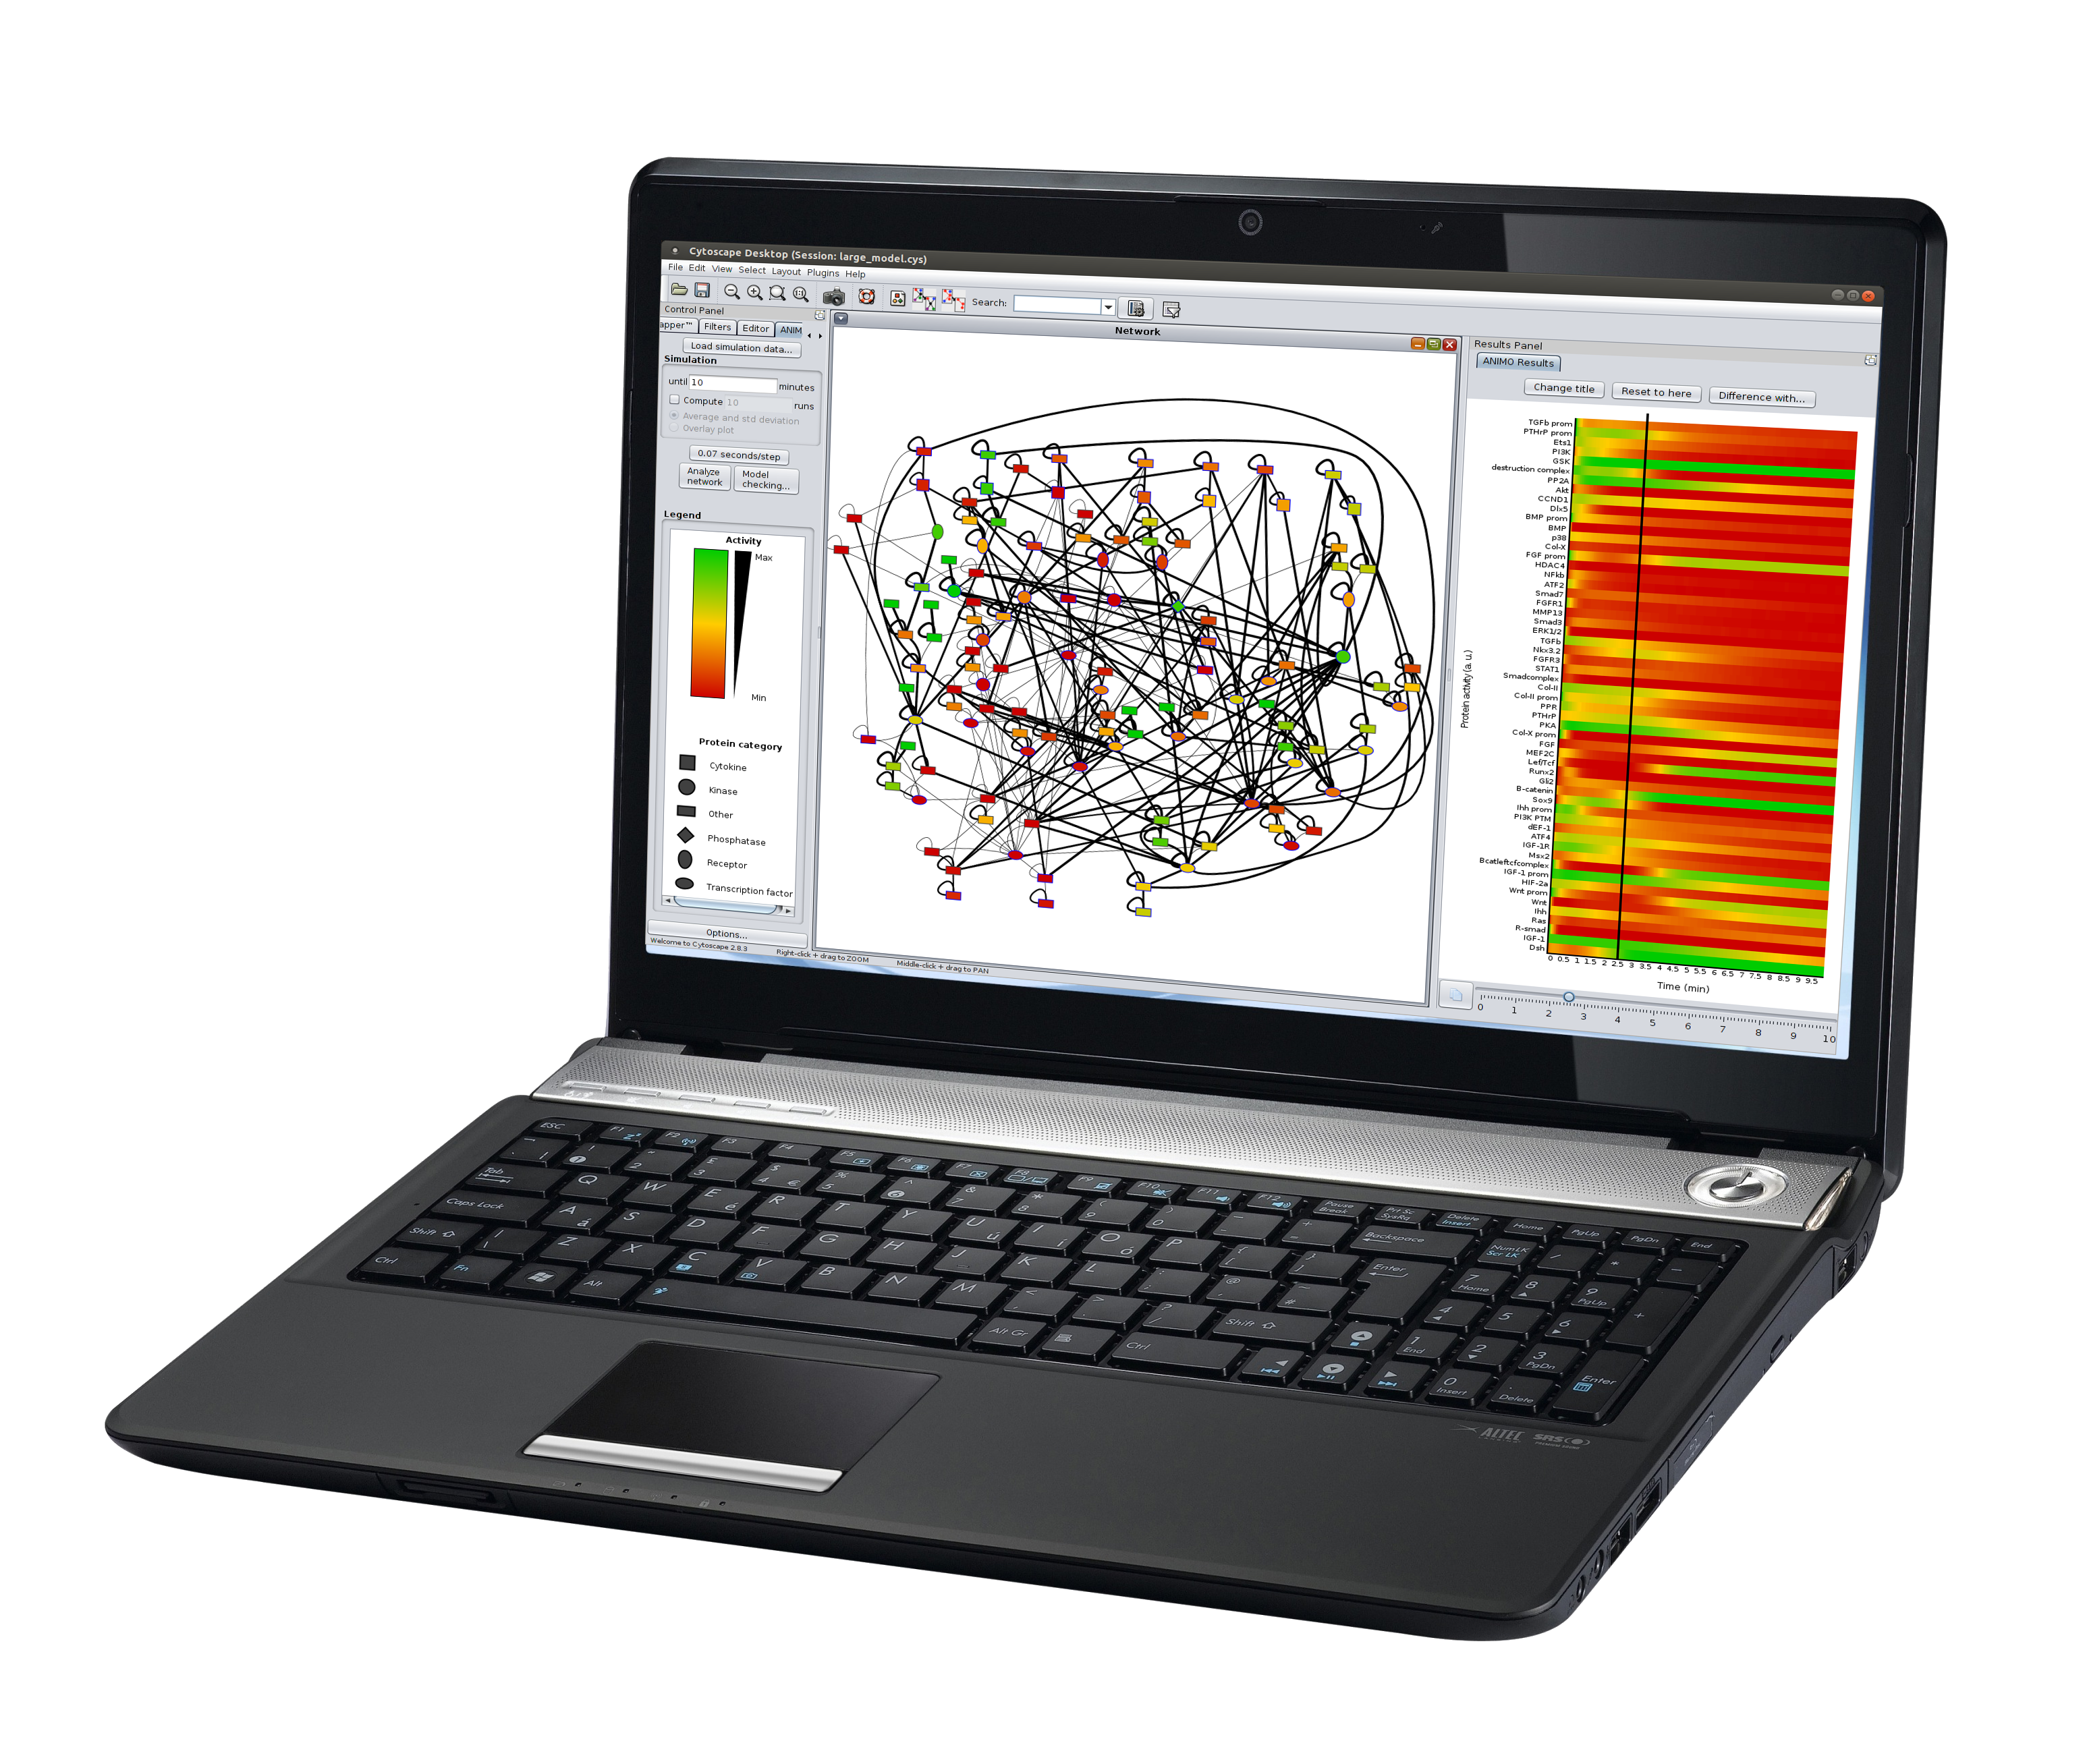
\includegraphics[width=0.8\textwidth]{images/animo_live_demo}
\end{center}
}

% \frame{ \frametitle{Case study: \emph{in silico} experiments}
%   \begin{center}
%     %  \begin{minipage}[c]{.9\textwidth}
%           \pgfuseimage{case-study}\\[-2ex]
%     %  \end{minipage}
%   \end{center}\vspace{-1ex}
%   {\tiny Model\vspace{-1.3ex} inspired by S. D. M. Santos, P. J. Verveer, and P. I. H. Bastiaens, ``Growth factor-induced
% MAPK network topology shapes Erk response determining PC-12 cell fate'', \emph{Nature Cell Biology}, Feb. 2007.}
% }

\frame{ \frametitle{Conclusions}
  \begin{itemize}
    \item<1-> Cytoscape $\rightarrow$ static representation,\\Timed Automata $\rightarrow$ dynamic behaviour
    %\item User interface based on Cytoscape: keep the complexity of Timed Automata \emph{under the hood}
    \item<2-> Discrete levels and simplified scenarios $\rightarrow$ few parameters
    %\item Underlying Timed Automata model provides formal foundations
    \item<3-> Modelling with ANIMO:\\
      \begin{itemize}
          \item outline pathway topology
          \item select reaction parameters
          \item compare model with existing data
          \item repeat until satisfied
      \end{itemize}
    \item<4-> ANIMO allows biologists to draw network ``sketches''
    \item<5-> Complex models:\\
      \begin{itemize}
	\item perform \emph{in silico} experiments
	\item use model checking
      \end{itemize}
  \end{itemize}
}

\frame[t]{ \frametitle{Future work}
  \begin{itemize}
%     \item Advance the development of user interface
%     \item Model checking queries:\begin{itemize} \item user-friendly (templates)
%     \item probabilistic (statistical model checking)
%     \end{itemize}
    \item<1-> Use \emph{in-silico experiments} to infer biological hypotheses which can be verified through in-vitro experiments
      \only<1-1>{\vspace{1ex}\\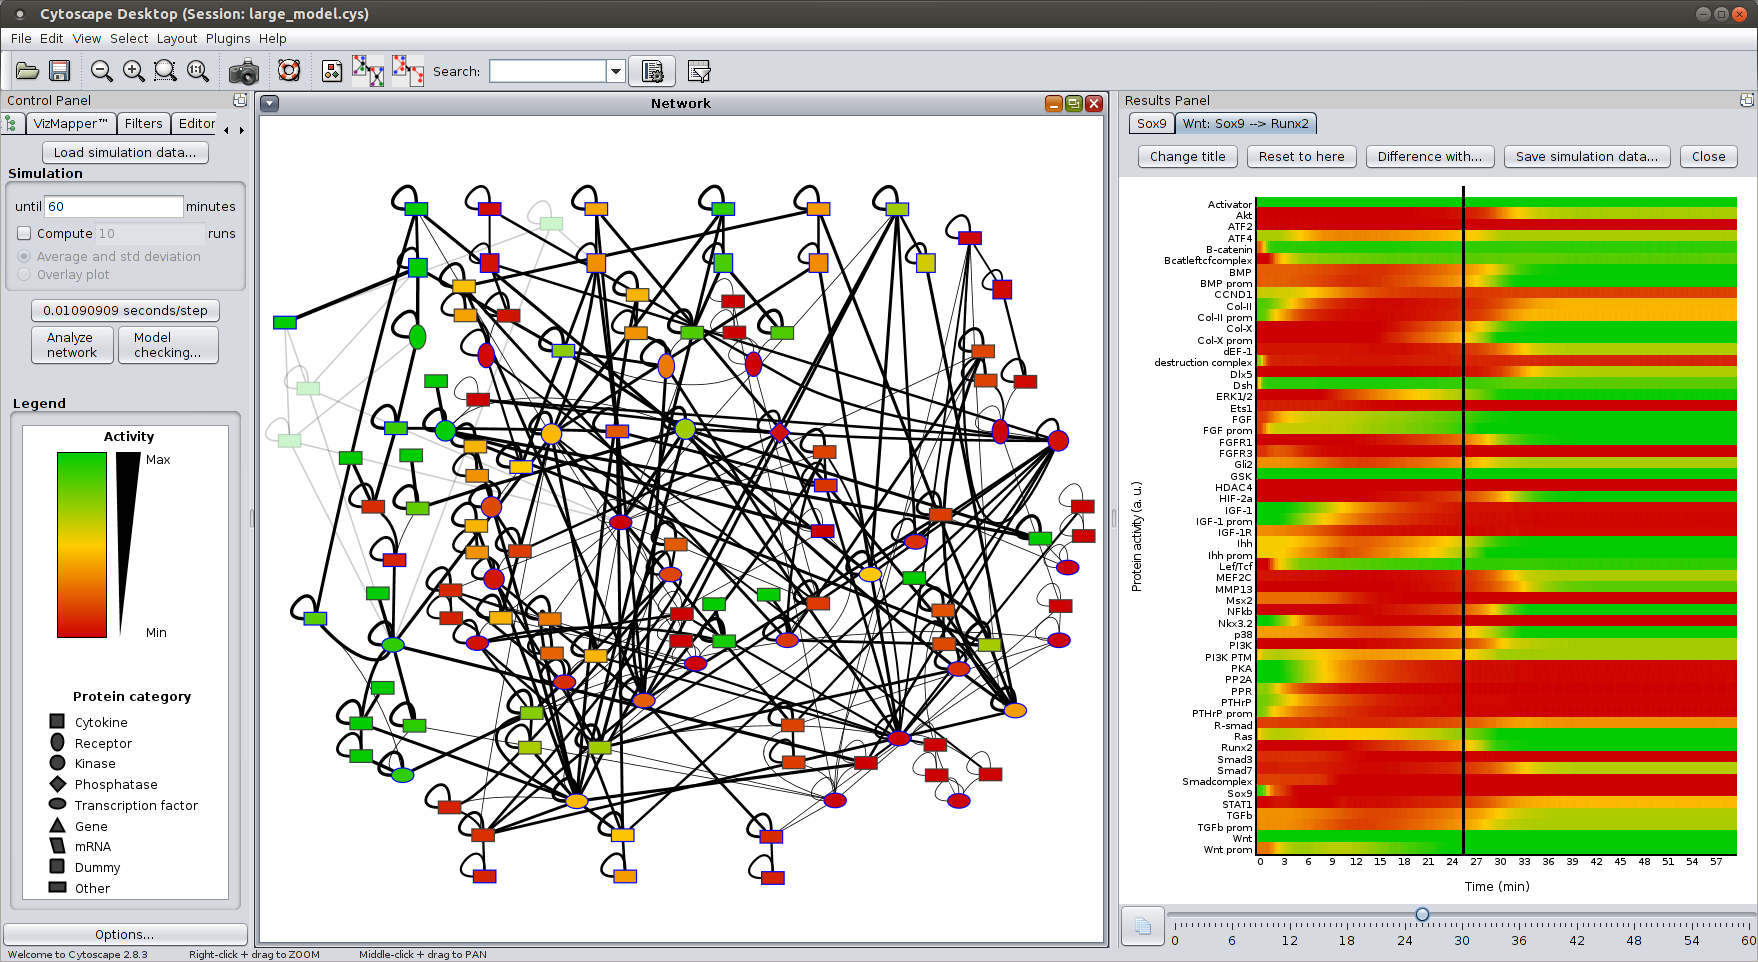
\includegraphics[width=0.95\textwidth]{images/large_model_sox9_runx2}}
    \item<2-> High-performance analysis of large models: multicore and distributed model checking
    \item<3-> Get a model by feeding data (proposal to NWO):\begin{itemize}
      \item Automata Learning to infer network topology from experimental data
      \item sensitivity analysis and parameter fitting
    \end{itemize}
    \item<4-> Abstraction techniques to deal with large models
  \end{itemize}
}

\frame{ \frametitle{Thank you}
  \begin{center}
      \pgfuseimage{animo-logo}\\
      Analysis of Networks with Interactive MOdelling\\[2ex]
      {\Large \url{http://fmt.cs.utwente.nl/tools/animo}}\\[1ex]
      \pgfuseimage{animo-qrcode}
  \end{center}
}

\end{document}
